\chapter{Acousto-optic intensity characteristics}

\textit{In the previous chapter we seeked for different aspects of the
\gls{rf} signal powering the \gls{aod} elements and found that the
electronic equipement provides an overall stable signal for the \gls{aod}.
In this chapter we want to examine the intensity characteristics subject
to frequency and amplitude parameters of the \gls{rf} signal. In the end
we will find that the intensity shows highly non-linear behaviour with
respect to the \gls{rf} signal parameters.}

\section{Intensity control}

The laser intensity is regulated by a control loop using an \gls{aom} in
order to compensate power drifts from the laser source. This control loop is
tightly integrated into our experimental setup \cref{ch:experimental_setup}
and thus will be present for all subsequent intensity measurements. Therefore
it is essential to check its stability and estimate its error contribution if
we want to interpret any other intensity related measurements.
\begin{figure}[ht]
  \centering
  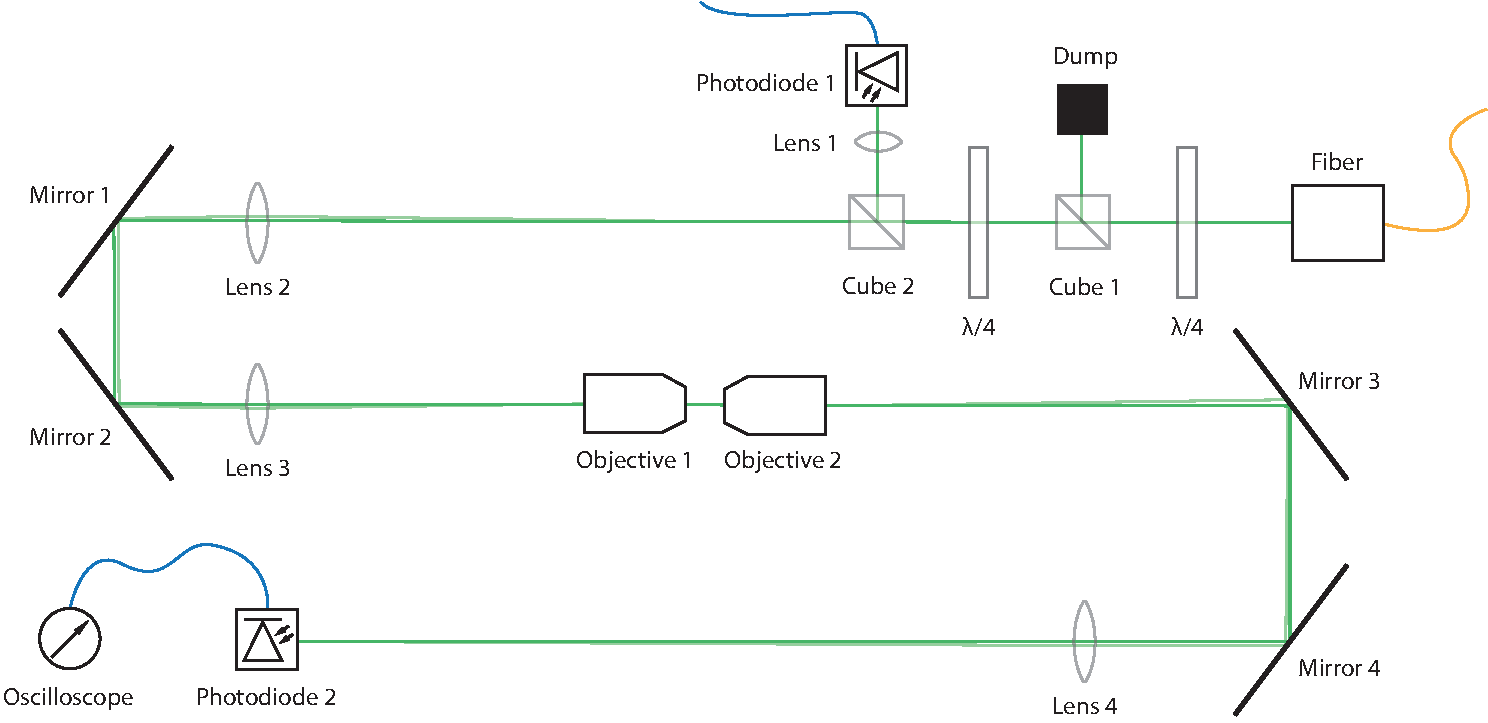
\includegraphics[width=.9\textwidth]{\mediadir{setup/intensity-control.pdf}}
  \captionsetup{width=.9\textwidth}
  \caption{Optical setup and intensity detection. The \gls{aod}s have been
    removed. The beam hits photodiode 2 that is connected to the oscilloscope.
  }\label{fig:intensity_control_setup}
\end{figure}
The experimental setup is the same as described in
\cref{ch:experimental_setup} but with disassembled \gls{aod} and Photodiode 2
at the terminus of the laser beam. The setup is depicted in
\Cref{fig:intensity_control_setup}. The intensity control via \gls{aom} is
placed in the power reduction setup from which the fiber originates. The
photodiode gain was set to \SI{50}{\decibel} if not otherwise noted.

\subsubsection{Long-term measurement}

We start by investigating the long-term behaviour of the intensity control
loop. In particular we look for oscillations or intensity collapses. Therefore
we measured the voltage of Photodiode 2 in an interval of about
\SI{2}{\minute} over a total time of approximately \SI{16}{\hour}.
\begin{figure}[ht]
  \centering
  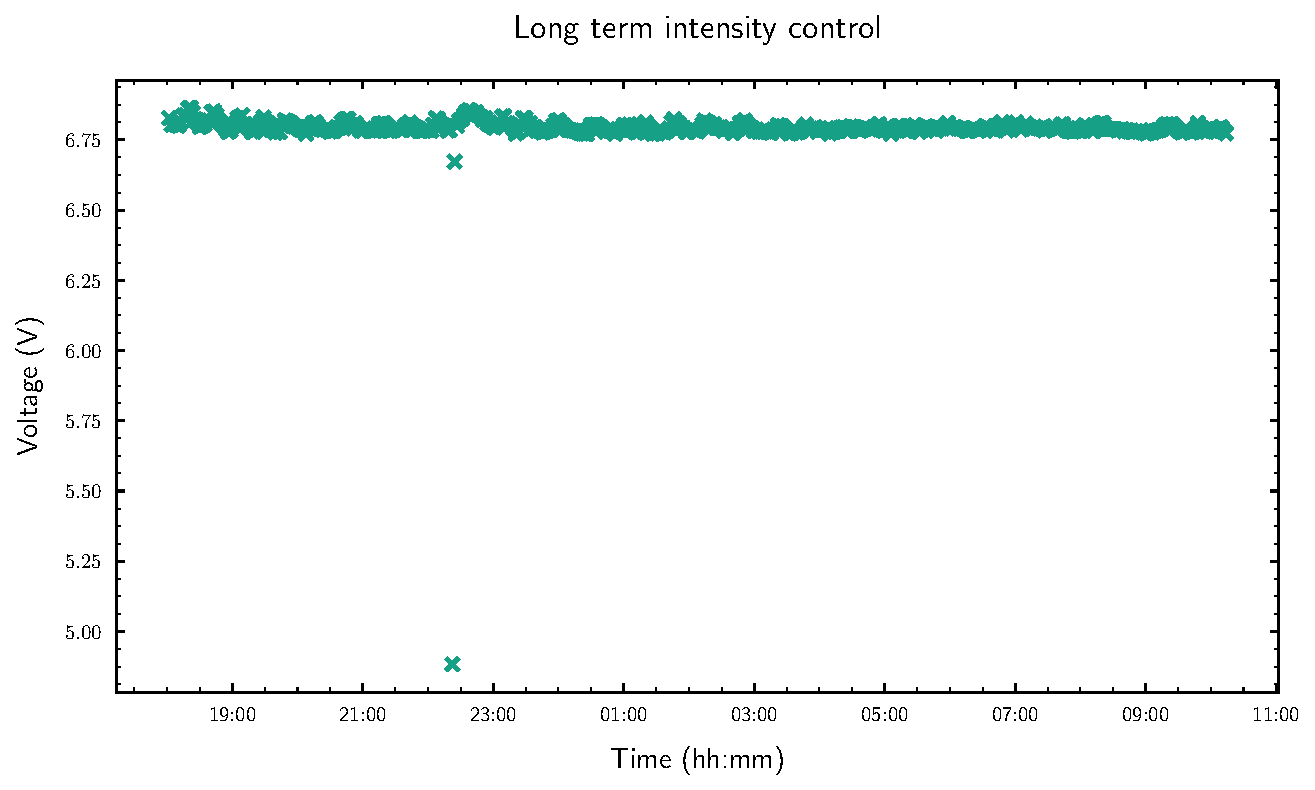
\includegraphics[width=\textwidth]{\figuredir{intensity/control/long.pdf}}
  \captionsetup{width=.8\textwidth}
  \caption{Long term measurement of the intensity with controlled intensity.
    The intensity was measured every \SI{2}{\minute} for over \SI{16}{\hour}
    to determine the accuracy of the intensity controller. The outlier at
    about 22:45 was caused by laboratory visit otherwise the intensity remains
  stable.}
  \label{fig:intensity_control_long}
\end{figure}
The voltage time series is shown in \Cref{fig:intensity_control_long}. We 
note outliers at about 22:45 which were caused by accidently interfering with
the setup during measurement. Further we see a constant albeit intensity
signal in contrast to the uncontrolled intensity signal where we could watch
real time oscillations and drifts. \Cref{tab:intensity_control_long} depicts
the descriptive statistics belonging to the voltage time series visualized in
\Cref{fig:intensity_control_long}. The mean intensity is measured to be around
\SI{6.79}{\volt} with peaks up to \SI{6.86}{\volt}. The standard deviation
yields us a relative error of around \SI{1.4}{\percent}.
\begin{table}[h]
  \centering
  \begin{tabular}{|c|c|c|c|}
    \hline
    Mean & Minimum & Maximum & Standard deviation \\
    \hline
    \SI{6.79}{\volt} &
    \SI{4.88}{\volt} &
    \SI{6.86}{\volt} &
    \SI{0.09}{\volt} \\
    \hline
  \end{tabular}
  \captionsetup{width=.8\textwidth}
  \caption{Descriptive statistics of the short term measurement of the
  intensity with controlled intensity. Note the small standard deviation.}
  \label{tab:intensity_control_long}
\end{table}

\subsection{Short-term measurement}

The previous section gave us already some good insights about the long term
stability of the intensity control loop. Yet in practice typical intensity
measurements are of much smaller magnitude, henceforth it seems close at hand
to also conduct a short term measurement.
\begin{table}[h]
  \centering
  \begin{tabular}{|c|c|c|c|}
    \hline
    Mean & Minimum & Maximum & Standard deviation \\
    \hline
    \SI{6.78}{\volt} &
    \SI{6.77}{\volt} &
    \SI{6.82}{\volt} &
    \SI{0.01}{\volt} \\
    \hline
  \end{tabular}
  \captionsetup{width=.7\textwidth}
  \caption{Descriptive statistics of the short term measurement of the
  intensity with controlled intensity. Note the small standard deviation.}
  \label{tab:intensity_control_short}
\end{table}
For the short term measurement time parameters were adjusted to a sample
interval of \SI{10}{\second} and measurment were performed over \SI{1}{\hour}.
\begin{figure}[ht]
  \centering
  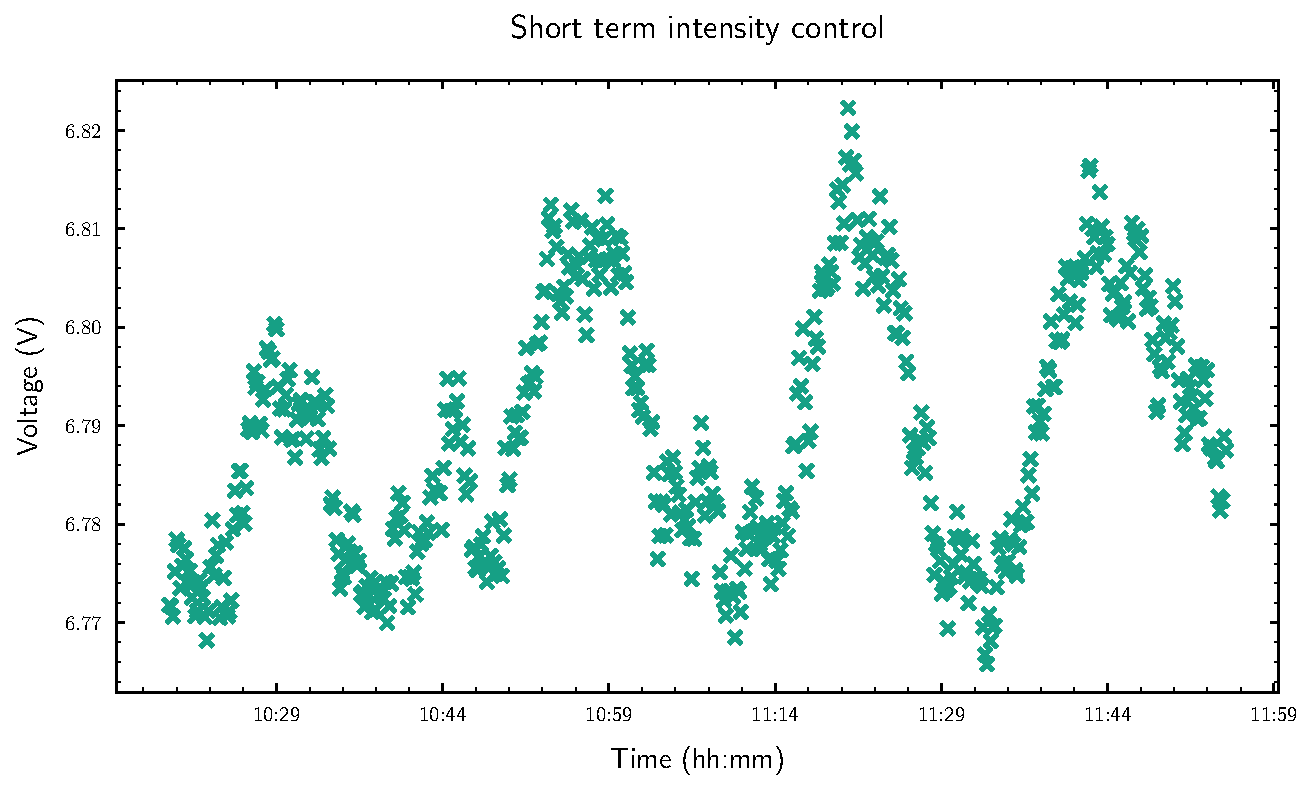
\includegraphics[width=\textwidth]{\figuredir{intensity/control/short.pdf}}
  \captionsetup{width=.8\textwidth}
  \caption{Short term measurement of the intensity with controlled intensity.
    The intensity was measured every \SI{10}{\second} for over \SI{1}{\hour}
    to determine the accuracy of the intensity controller.}
  \label{fig:intensity_control_short}
\end{figure}
The intensity time series of the short term measurement is depicted in
\Cref{fig:intensity_control_short} and the associated descriptive
statistics are presented in \Cref{tab:intensity_control_short}.

On a smaller timescale we see that the intensity control loop performs
periodic oscillations, however the descriptive statistics show much smaller
deviation from the mean, than observed in the long term measurements. As we
do not see outliers in \Cref{fig:intensity_control_short} we can pay more
attention to the value range of \SI{0.05}{\volt} which was obfuscated in
the long term measurement because of outliers.

\subsubsection{Summary}

The previous discussion confirmed that the intensity is regulated in that
we only observe oscillations around the targeted intensity value. Yet we are
still missing statements with regard to the magnitude of these oscillations
as we are missing a comparison to real intensity data.

\begin{table}[h]
  \centering
  \begin{tabular}{|c|c|c|}
    \hline
    Measurement & Value range & Standard deviation \\
    \hline
    long term & \SI{1.98}{\volt} & \SI{0.09}{\volt} \\
    \hline
    short term & \SI{0.06}{\volt} & \SI{0.01}{\volt} \\
    \hline
    typical & \SI{1.43}{\volt} & \SI{0.40}{\volt} \\
    \hline
  \end{tabular}
  \captionsetup{width=.8\textwidth}
  \caption{Descriptive statistics of the short and long term measurement
  of the intensity control and a typical intensity measurements where we
subtracted the mean intensity for comparison.}
  \label{tab:intensity_control}
\end{table}

For a typical measurement, to compare the intensity oscillations with, we
elected the intensity progression of a linear frequency sweep of the
\gls{aod} in the vertical socket while the \gls{aod} in the horizontal socket
is fixed. We will discuss this specific meausurement in detail in a later
section. In \Cref{tab:intensity_control} we see some statistics of the
long and short term measurements next to the typical measurement.

\begin{figure}[ht]
  \centering
  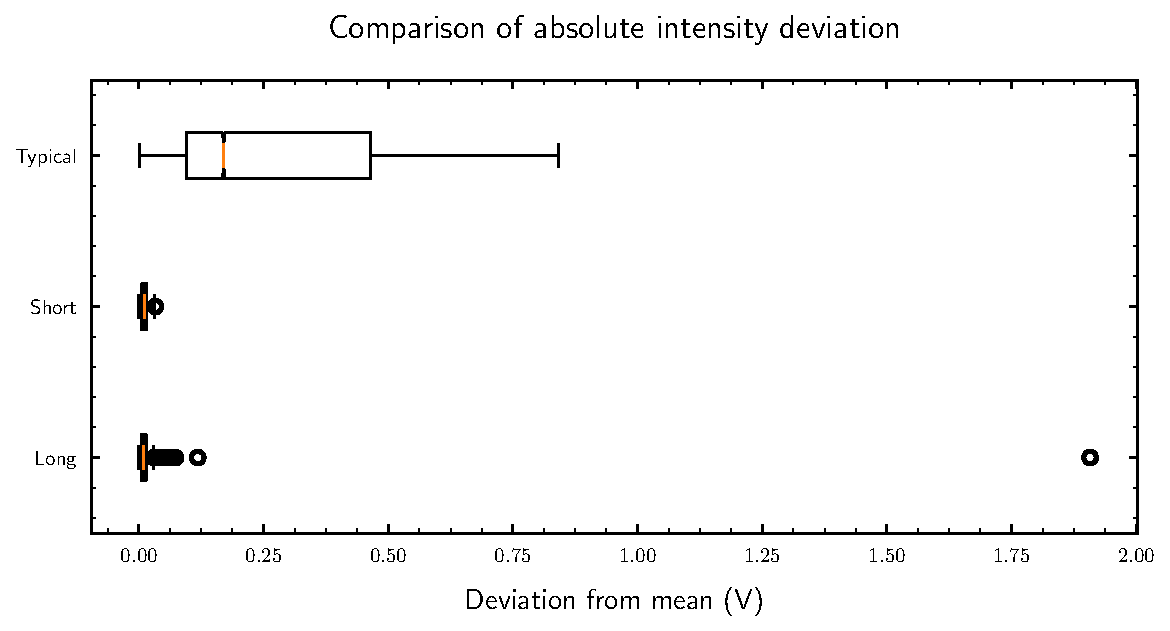
\includegraphics[width=\textwidth]{\figuredir{intensity/control/deviation.pdf}}
  \captionsetup{width=.8\textwidth}
  \caption{Boxplot of the long and short term intensity measurements and a typical
  intensity measurement with the \gls{aod} where we subtracted the mean intensity
  for comparison. The typical measurements covers a much wider intensity range
then deviations from the intensity control loop.}
  \label{fig:intensity_control_comparison}
\end{figure}

One dismally error estimate would be the quotient of the value range of the
short term measurement and the typical measurement, yielding an error of
\SI{4.2}{\percent}. A second approach would be the quotient of the standard
deviation of the short term and typical measurement, yielding
\SI{2.5}{\percent} error. When comparing the typical measurement to the
statictis of a long term measurement we find rather large errors which
suggests that there re other statistical key figures which may be more
suitable.

A boxplot is very useful in visualizing the spread. We have an orange stripe
marking the median, the contour of the box marking the data between first and
third quantil. The usual value range is marked by the whiskers and outliers
are marked as the circles outside the whiskers.
In \Cref{fig:intensity_control_comparison} we see such a boxplot for the
absolute deviation from the mean of the three measurements. The absolute
deviation from the mean accounts for the different transmission just because
of the presence of the \gls{aod} in the typical measurement but keeps the
linear scale unlike the squared deviation from mean. We can see that in a
typical measurement (upper boxplot) the usual deviation from mean is much
larger than for the short and long term measurement of the intensity
regulation.

\section{Spatial beam profile}

We figured out that the intensity control loop operates as expected. Next we
want to assess the quality of our optical alignment to sort out later
systematic measurement errors from poor calibration. One way to assess the
alignment grade of our alignment is to evaluate the spatial profile of the
laser beam with respect to deviations from an ideal gaussian profile.

\subsubsection{Experimental setup}

In the previous setup we used a second photodiode to measure the temporal
deviations of the intensity. In order to measure spatial deviations of the
intensity we replaced the photodiode with a \gls{ccd} camera.

\begin{figure}[ht]
  \centering
  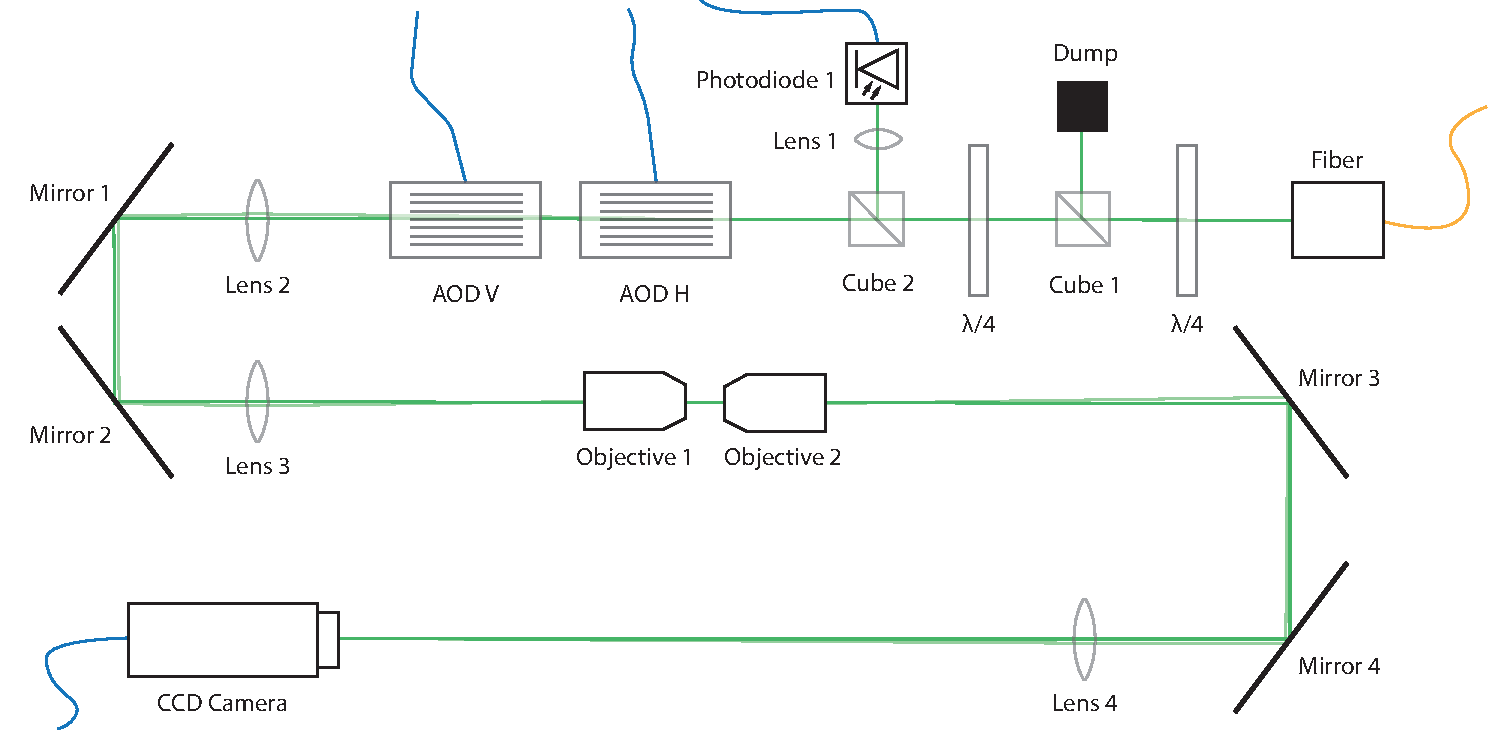
\includegraphics[width=\textwidth]{\mediadir{setup/intensity-profile.pdf}}
  \captionsetup{width=.8\textwidth}
  \caption{The beam is focused onto the \gls{ccd} sensor of the camera. The
    \gls{aod} are configured at \SI{100}{\mega\hertz} center frequency.
  }
  \label{fig:intensity_profile_setup}
\end{figure}

In \Cref{fig:intensity_profile_setup} we see the setup used to measure the
beam profile. The \gls{aod} are configured at \SI{100}{\mega\hertz} center
frequency. The distance between Lens 4 and the \gls{ccd} sensor is chosen
such that the the beam head is focused.

In \Cref{fig:intensity_profile_2d} we can see an enlarged image patch of the
complete image caputre taken with the \gls{ccd} camera. We can see a strong
illuminated circular spot in the center of the iamge with an area of about
\SI{2.5}{\milli\meter}. The intensity inside the spot seems homogeneous,
however this is caused because the pixels are saturated in this area.
We could reduce the intensity or apply an optical filter to the camera to
resolve the intensity gradient inside the spot, but only at the cost of
the intensity distribution around the spot. Around the circular spot we can
see a diffraction ring. The diffraction ring is well described in
\cite{Hertlein2017} and originates from the finite aperture of the objectives.

\begin{figure}[ht]
  \centering
  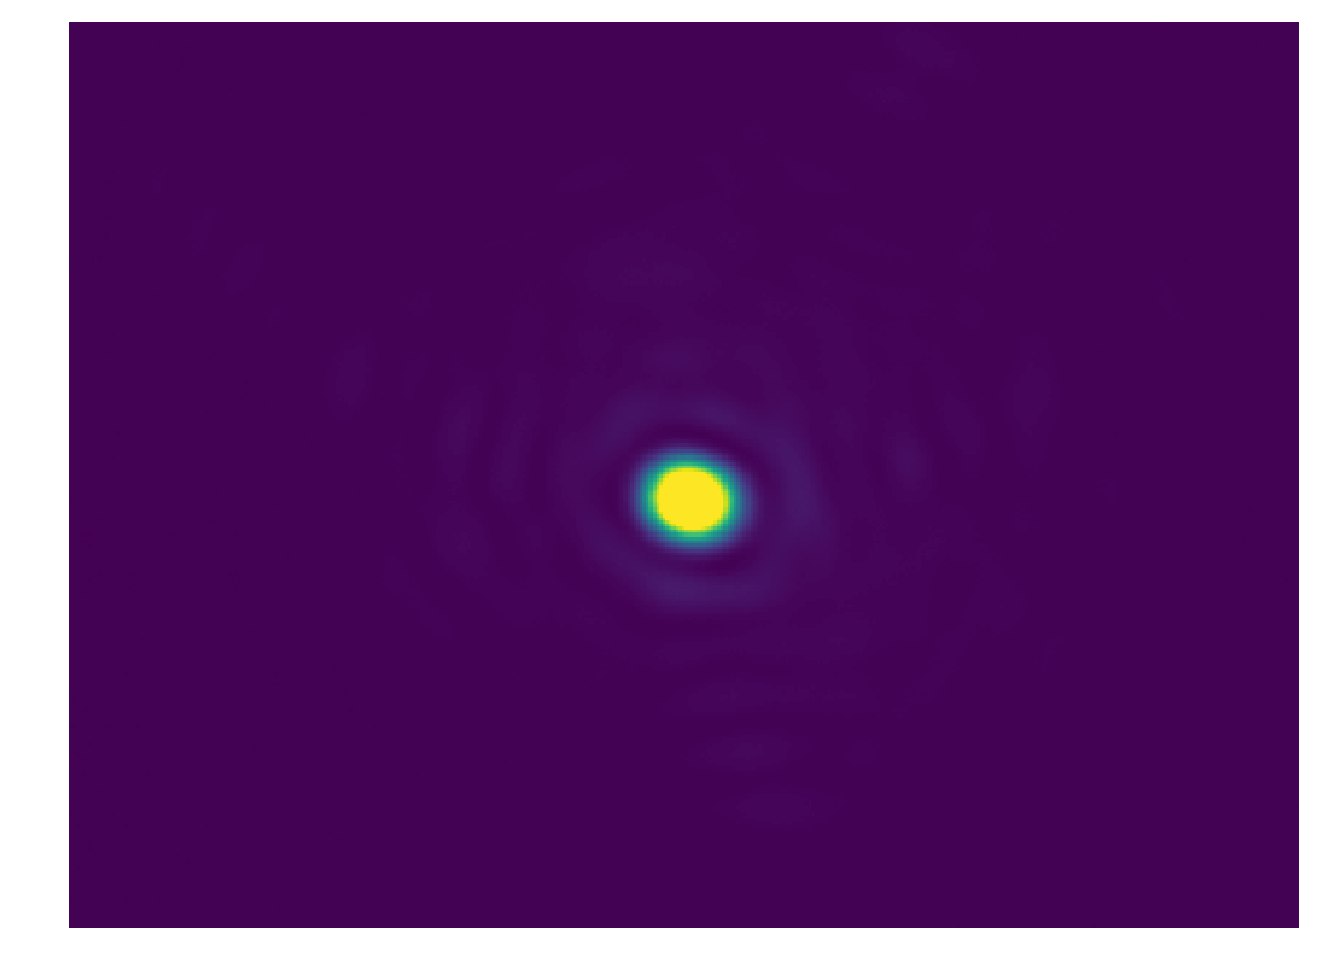
\includegraphics[width=.5\textwidth]{\figuredir{intensity/profile/profile2d.pdf}}
  \caption{Image detail from the captured beam with the \gls{ccd} camera.}
  \label{fig:intensity_profile_2d}
\end{figure}

Altough \Cref{fig:intensity_profile_2d} gives us a good overview of the
spatial beam profile it is difficult to see deviations from an ideal
gaussian curve in this representation. Henceforth we performed two
perpendicular cuts and visualized the one dimensional spatial beam
distribution in \Cref{fig:intensity_profile_1d}.

\begin{figure}[ht]
  \centering
  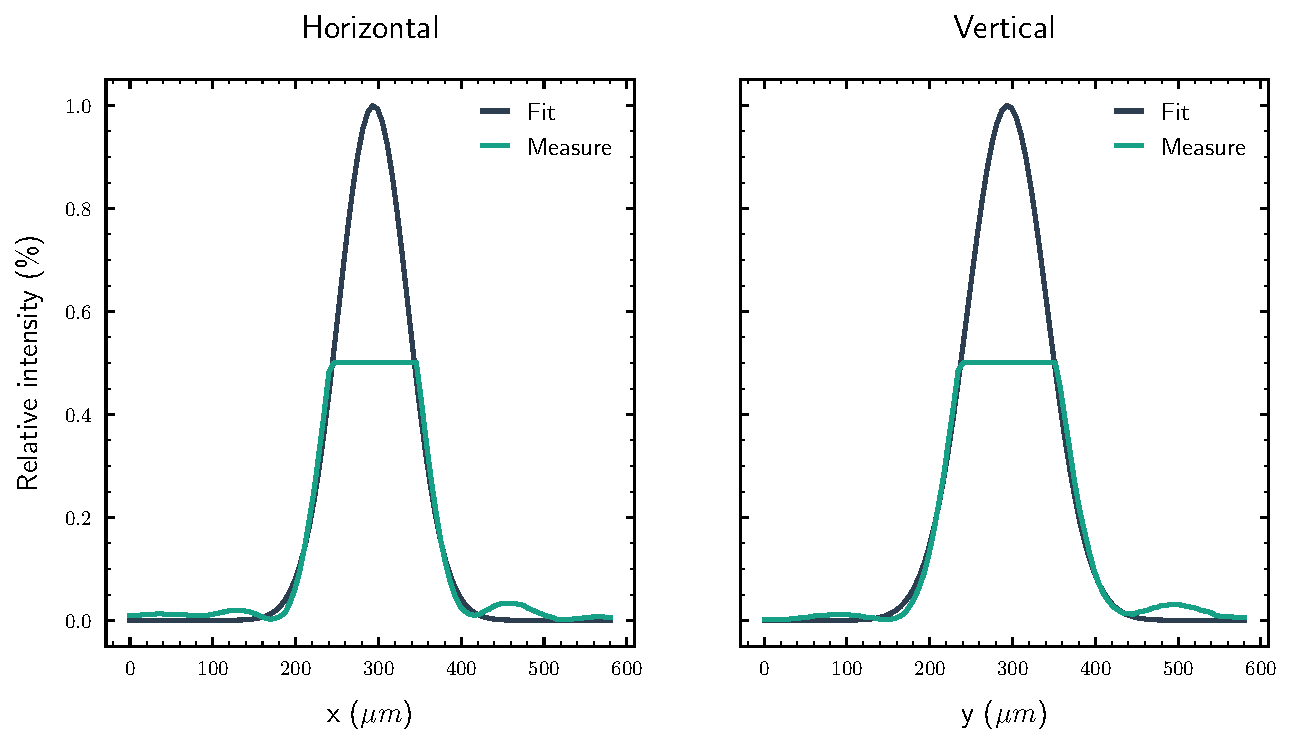
\includegraphics[width=\textwidth]{\figuredir{intensity/profile/profile1d.pdf}}
  \captionsetup{width=.8\textwidth}
  \caption{One dimensional perpendicular cut of the two dimensional beam
    distribution from the two dimensional beam profile in
    \cref{fig:intensity_profile_2d} with fitted gaussian curve.}
  \label{fig:intensity_profile_1d}
\end{figure}

In \Cref{fig:intensity_profile_1d} we can clearly observe the effects of
saturation around the center and how we would expect the intensity to be
if we could experimentally resolve it in the Gaussian fit. In contrast to the
ideal Gaussian profile we again observe contributions to the Airy disc around
the otherwise Gaussian profile causes by the finite aperture. Further we can
now clearly observe assymmetry from the intensity contributions around the
Gaussian which means that our alignment is not perfect.

\subsubsection{Summary}

We can confirm the results reported in \cite{Hertlein2017} that the spatial
beam profile equals a two dimensional Gaussian combined with a diffraction
ring caused from the finite aperture of the objectives. Further we observe
slight assymmetries in the diffraction ring suggesting inperfect alignment.

Though assymetries in the spatial beam profile are present, we do not see any
further complications as the intensity measurements with the photodiode will
cover the complete beam profile.

\section{Difference between individual acousto-optic deflectors}

Our optical setup uses a single two dimensional \gls{aod} that comprises two
\gls{aod} elements perpendicular to eachother. At first we want to examine the
behaviour of the single \gls{aod} elements to eachother. In particular we
are interested if and how the \gls{aod} elements differ.

\subsubsection{Experimental setup}

The used 2D \gls{aod} is depicted in \Cref{fig:aod_socket}. We see the
two \gls{aod} elements in the respective horizontal and vertical slot. The
internals of the vertical \gls{aod} (left-hand side) are illustrated. The
element itself spans through the casing (dashed line) while the acousto-optic
crystal (dotted line) is glued onto the element. The laser beam passes through
the acousto-optic crystal. In the following we will refer to the horizontal
\gls{aod} element as the \gls{aod} element anticipated for the horizontal
slot and accordingly to the vertical \gls{aod} element as the \gls{aod}
element intended for the vertical \gls{aod} socket.

\begin{figure}[ht]
  \centering
  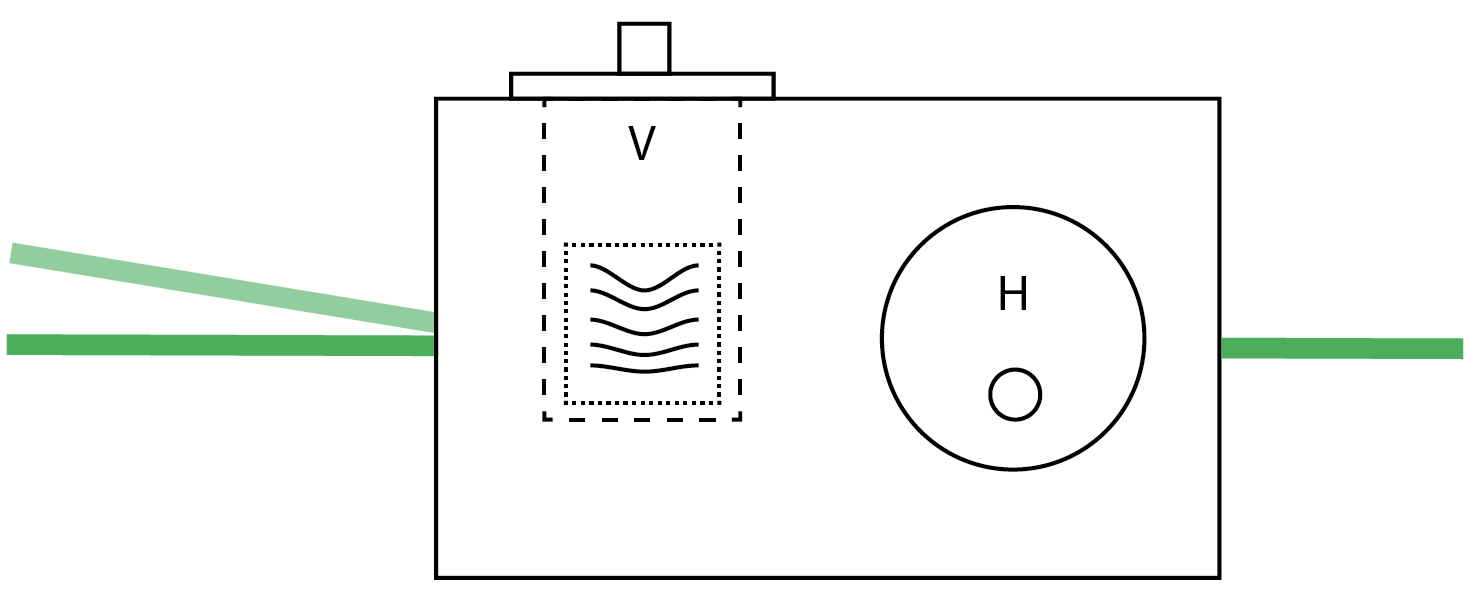
\includegraphics[width=\textwidth]{\mediadir{setup/aod-socket.png}}
  \captionsetup{width=.8\textwidth}
  \caption{The 2D \gls{aod} comprises two perpendicular orientated \gls{aod}
  elements.}
  \label{fig:aod_socket}
\end{figure}

\subsection{Individual acousto-optic deflectors}

For the following experiment we will only leave one \gls{aod} element mounted
in the casing depicted in \Cref{fig:aod_socket}. The other slot will be empty.
Then we will exchange socket positions for each respective \gls{aod} element
and measure the beam intensity subject to the linear frequency sweep from
\SI{80}{\mega\hertz} to \SI{120}{\mega\hertz} over a duration of
\SI{260}{\milli\second} and the configured \gls{dds} amplitude. As \gls{rf}
signal source the amplifier and \gls{dds} combination intended for the
horizontal \gls{aod} element was used to avoid influences of the amplification
offset between the two amplifiers.

The result for the four configurations (horizontal element in horizontal slot,
horizontal element in vertical slot, vertical element in horizontal slot
and vertical element in vertical slot) are visualized as heatmaps in
\Cref{fig:intensity_distribution_unpaired}. The color values are normalized in between the
different heatmaps and can be related to the measured voltage from the
photodiode by the colorbar on the right-hand side.

\begin{figure}[ht]
  \centering
  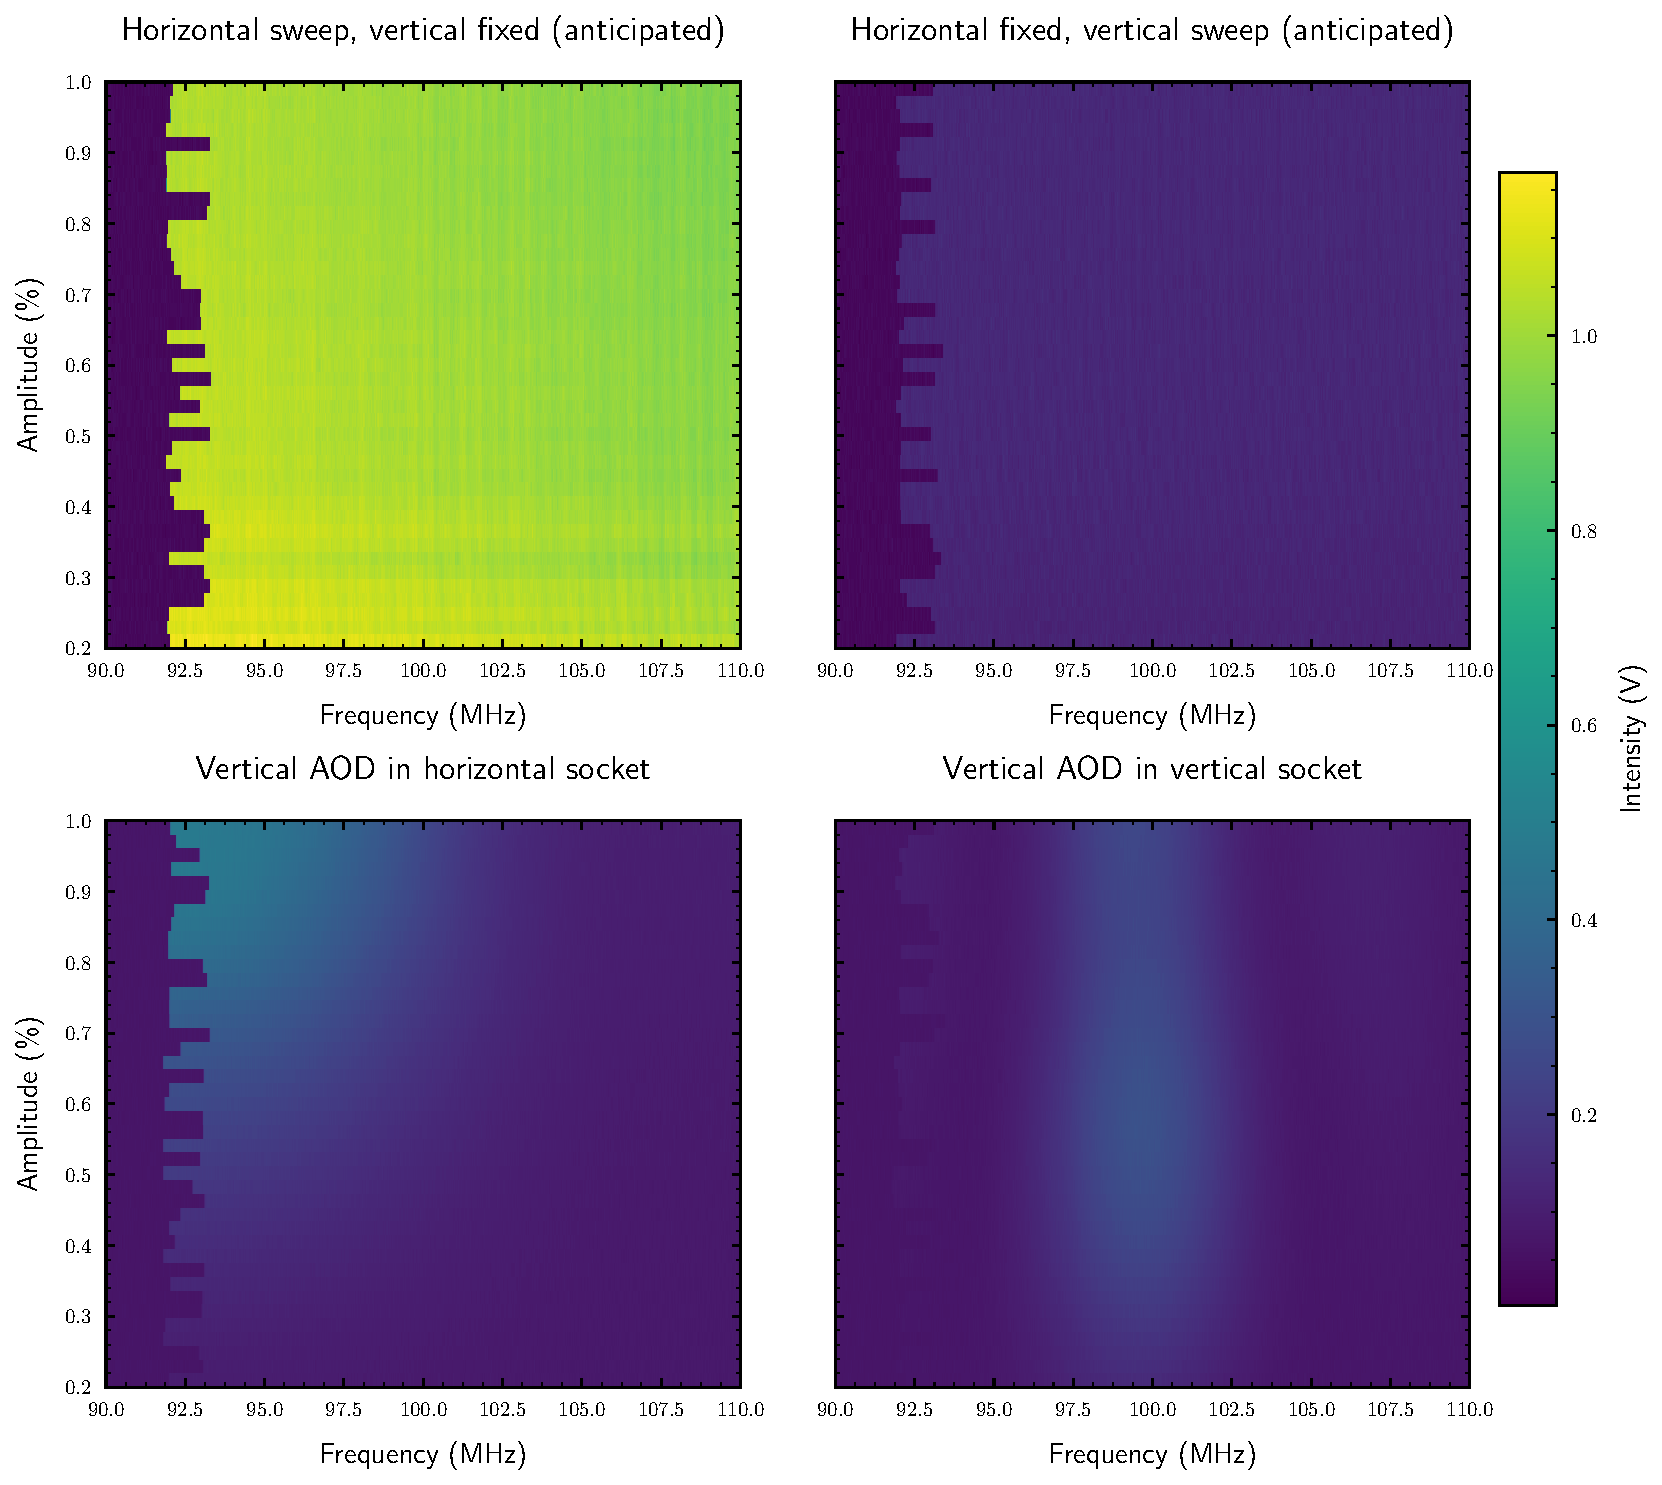
\includegraphics[width=\textwidth]{\figuredir{intensity/distribution/unpaired-amplitude.pdf}}
  \captionsetup{width=.8\textwidth}
  \caption{Intensity distribution over linear frequency sweep at different
  configured \gls{dds} amplitudes for different individual \gls{aod}
configurations.}
  \label{fig:intensity_distribution_unpaired}
\end{figure}

Oddly enough we observe that both \gls{aod} differ strong in their respective
intensity transmission behaviour in dependence of their slot position.
Furthermore we observe that the intensity transmission is much higher in the
case of the horizontal \gls{aod} element mounted to the intended horizontal
slot compared to all other configurations. In addition we can see that for
the horizontal \gls{aod} has an asymmetric, probably non-analytic, intensity
transmission. The highest intensity transmission is obtained for relative
amplitudes configured between \SI{60}{\percent} and \SI{90}{\percent} with
high dependence on the frequency. Another interesting observation is that
the intensity transmission seems very similar for the horizontal element in
the vertical slot and the vertical element in the vertical slot which
map also seems more symmetric with respect to the frequency axis. In fact
for these configurations the configured relative amplitude seems not to
interfere much with the measured voltage at the photodiode.

\subsection{Paired acousto-optic deflectors}

The \gls{aod} elements differ significantly in their intensity transmission
in between and with respect to their position. We find the horizontal element
in the anticipated horizontal position to have a significantly higher
transmission then any other configuration. Therefore we presume that the
\gls{aod} elements have a very high polarization dependency and are concerted
to eachother. We may find more evidence for this hypothesis by mounting both
\gls{aod} elements in their intended and exchanged slots.

\begin{figure}[ht]
  \centering
  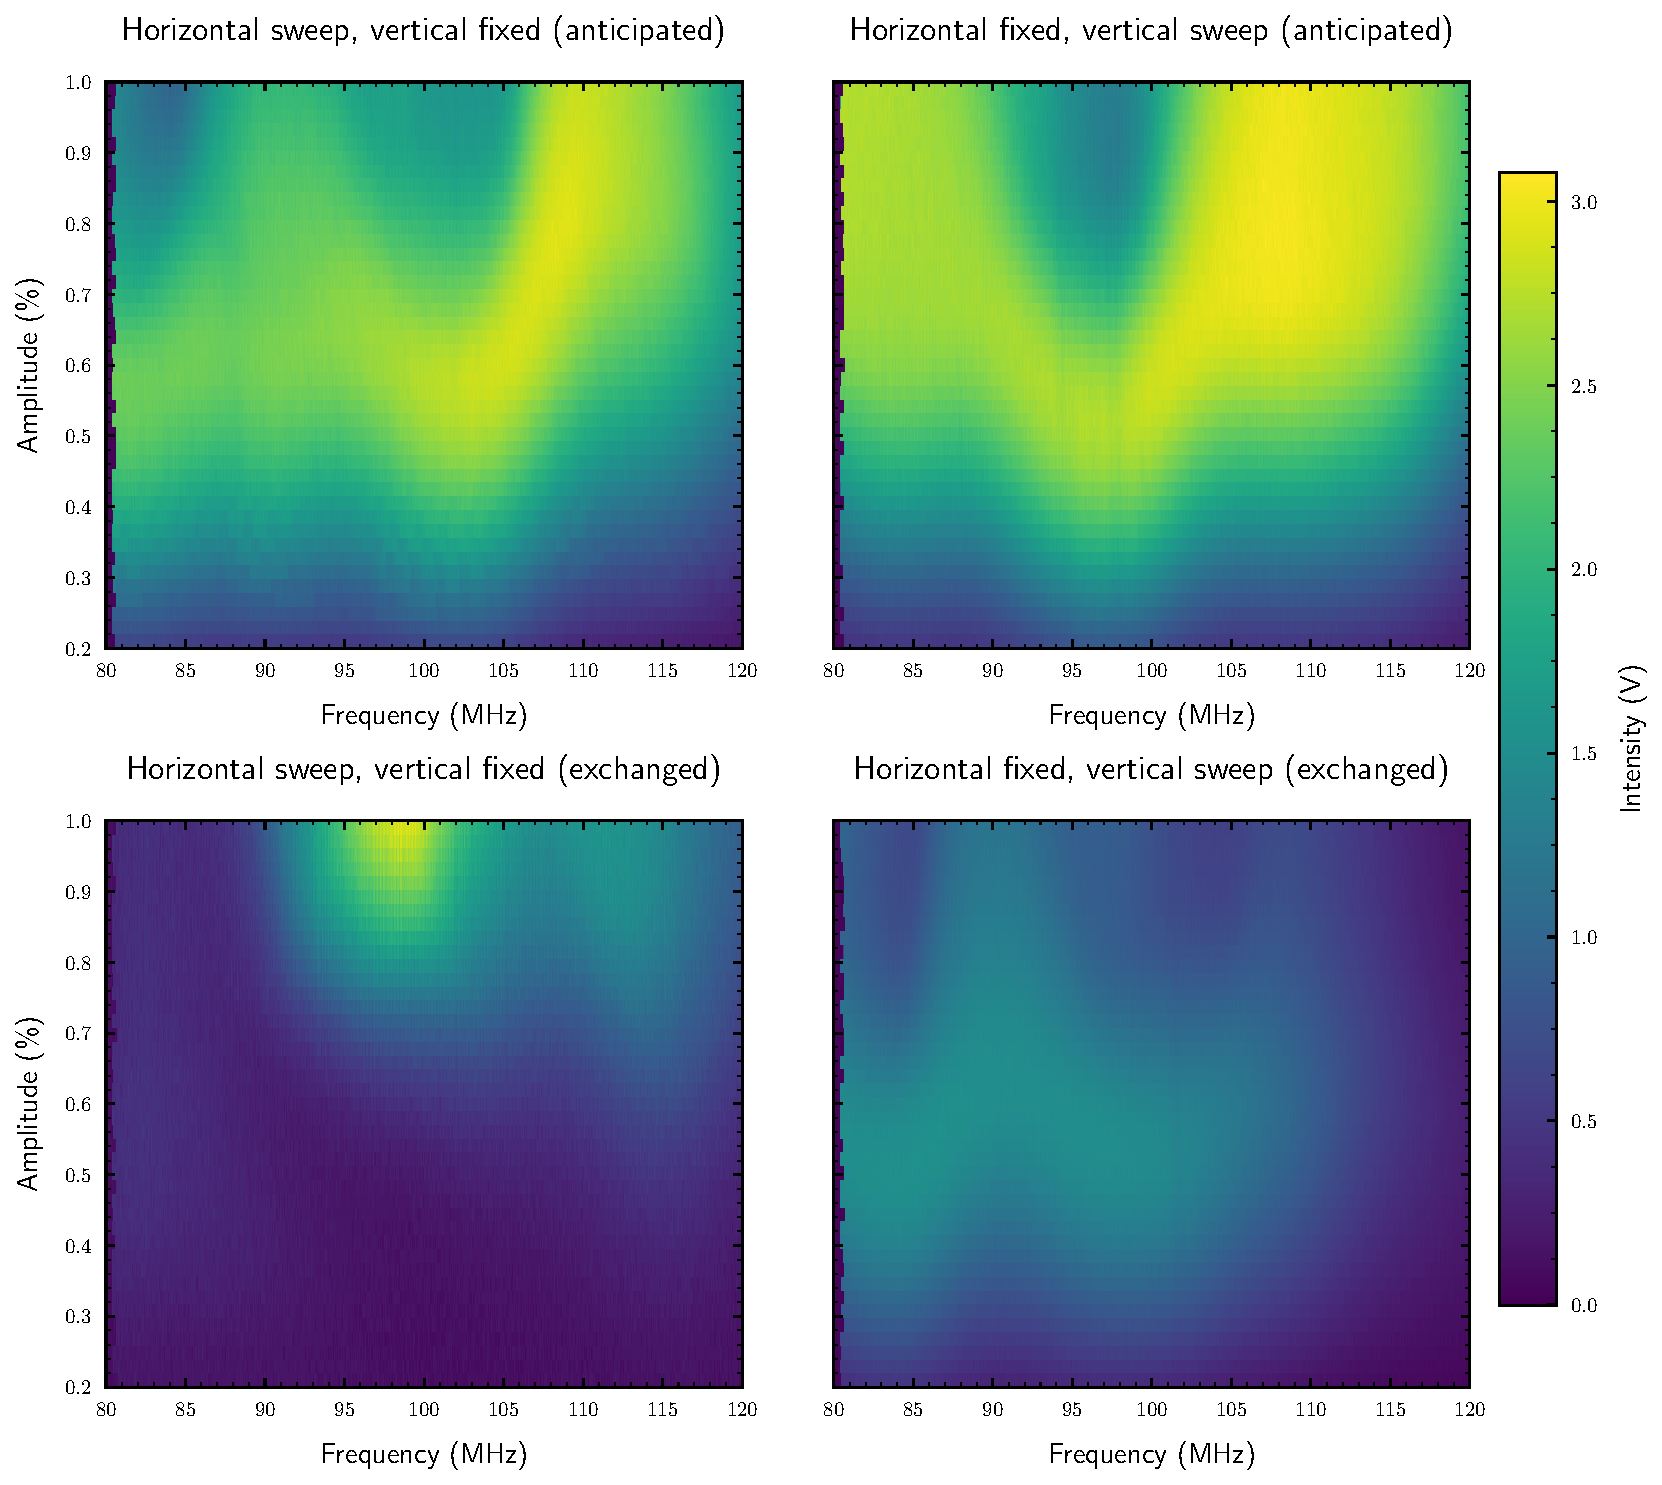
\includegraphics[width=\textwidth]{\figuredir{intensity/distribution/paired-amplitude.pdf}}
  \captionsetup{width=.8\textwidth}
  \caption{Intensity distribution over linear frequency sweep at different
  configured \gls{dds} amplitudes for different individual \gls{aod}
configurations.}
  \label{fig:intensity_distribution_paired}
\end{figure}

In \Cref{fig:intensity_distribution_paired} the measured voltage of the
second photodiode are visualized in a two-dimensional heatmap. The horizontal
axis represents the frequency of the \gls{rf} signal applied to the \gls{aod}
elements whereas the vertical axis the configured \gls{dds} relative
amplitude. In the first row the elements where in their intended slots whereas
we exchanged them for the second row. In the first column the frequency
sweep was applied such that the beam moves along the horizontal axis while
in the second column the frequency sweep was applied to the element that
causes beam movement in the vertical direction.

We see that for the exchanged positions the transmission is reduced and
asymmetric with respect to the sweep direction whereas the elements in their
intended position perform better in every aspect. We therefore conclude that
the \gls{aod} are cut in a intended way to account among others for
polarization effects and it is advised to operate them in their anticipated
slot as we will do for all following experiments.

\subsubsection{Summary}

The transmission of \gls{aod} crystals depends among others on the
polarization mode of the incident laser beam. A two dimensional \gls{aod}
has to be designed around this property and therefore requires the crystals
to be matched to each other.

\section{2D intensity distribution}

In the previous section we sorted out the influence of the \gls{aod} element
position and acknowledged that \gls{aod}s differ significant in their
optical properties. In the present section we now want to explore the
intensity transmission for a two dimensional sweep as intended to be used
for the optical potentials.

\subsubsection{Experimental setup}

The experimental setup is similar to the previous setups and is shown in
\Cref{fig:intensity_distribution_setup}. We have both \gls{aod} mounted in
their anticipated position. The \gls{aod} elements are aligned to maximize
intensity at the center frequency. The laser beam is directed into a second
photodiode where we measure the intensity with respect to the configured
\gls{dds} signal.

\begin{figure}[ht]
  \centering
  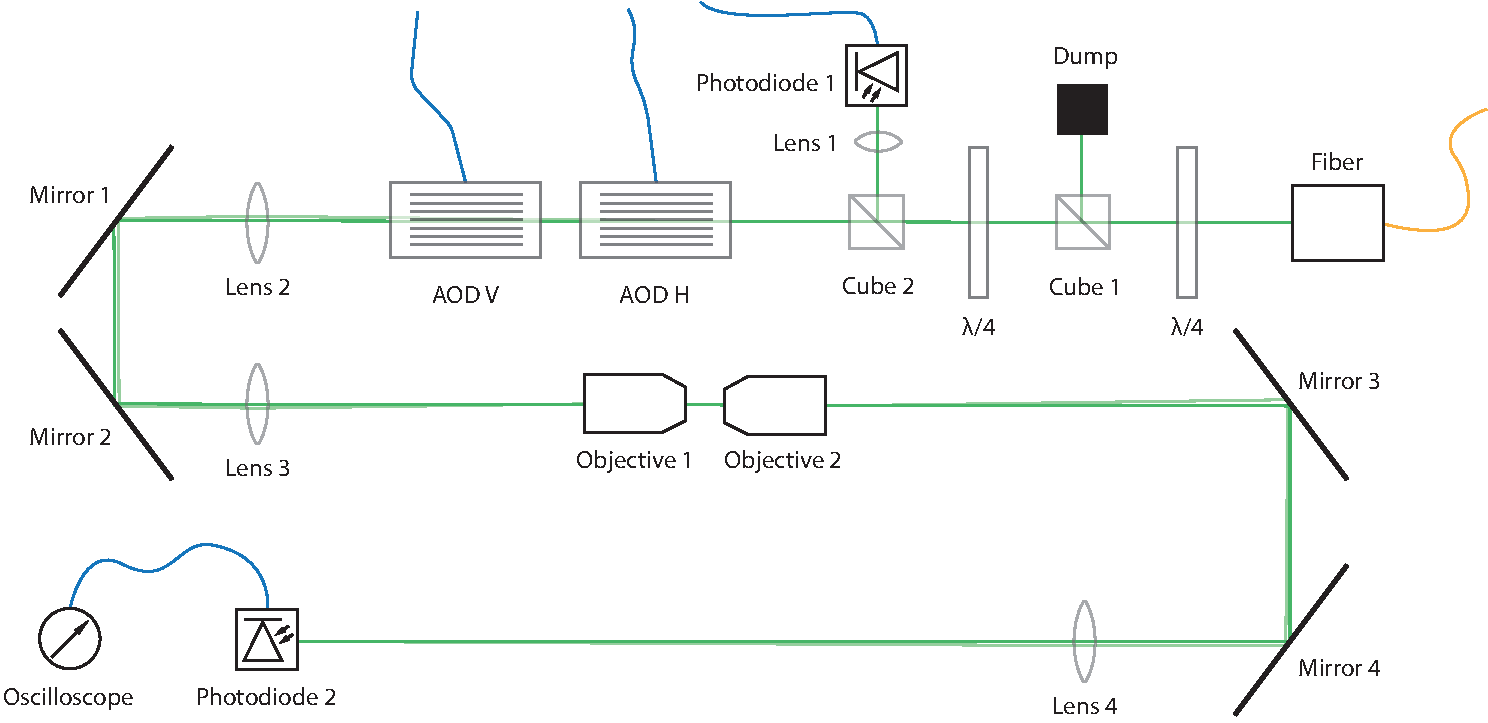
\includegraphics[width=\textwidth]{\mediadir{setup/intensity-distribution.pdf}}
  \captionsetup{width=.8\textwidth}
  \caption{Experimental setup used to measure the intensity transmission of
  the 2D \gls{aod} in dependence of the configured \gls{dds} signal.}
  \label{fig:intensity_distribution_setup}
\end{figure}

\subsubsection{Digital ramp frequency sweep}

In a first attempt we configure a first \gls{dds} to output a constant
frequency whereas a second \gls{dds} is configured to do a frequency sweep
using the internal digital ramp. After one such sweep the constant frequency
output of the first \gls{dds} is increased and the measurement repeats. The
procedure is repeated until the first \gls{dds} covered the same frequency
range as the second \gls{dds} per measurement.

\begin{figure}[ht]
  \centering
  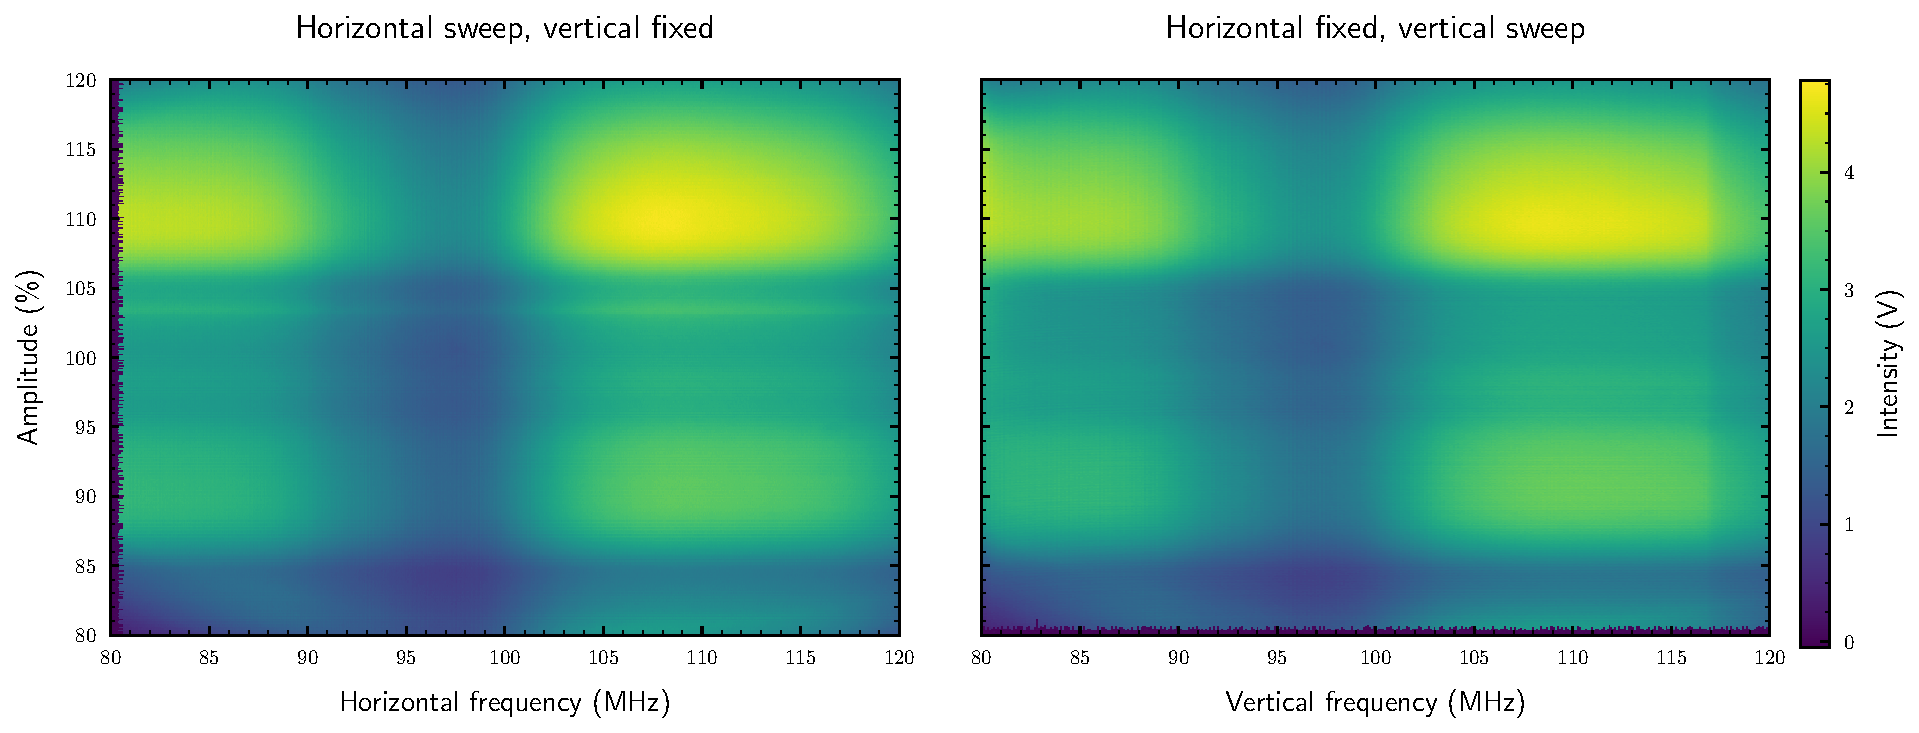
\includegraphics[width=\textwidth]{\figuredir{intensity/distribution/paired-frequency.pdf}}
  \captionsetup{width=.8\textwidth}
  \caption{Intensity measured as voltage at the photodiode in dependence of
    the horizontal and vertical applied frequency signal to the \gls{aod}. The
    left map is obtained by enabling the digital ramp on the horizontal
    \gls{dds} whereas the vertical \gls{dds} is configured to output a
    constant frequency which is manually increased after each measurement.
    On the right-hand side map the roles are exchanged.}
  \label{fig:intensity_distribution_frequency}
\end{figure}

In \Cref{fig:intensity_distribution_frequency} we are presented the intensity
measured at the second photodiode in the setup shown in
\Cref{fig:intensity_distribution_setup}. On the left-hand map the first
\gls{dds} is the \gls{dds} responsible for translations in vertical direction
whereas the second \gls{dds} is responsible for translations in horizontal
direction. This fact is also represented in the dimensionality of the
measurement data and can be observed at a close glance where we can see the
stripes in the direction of the more densely performed sweep.

\begin{figure}[ht]
  \centering
  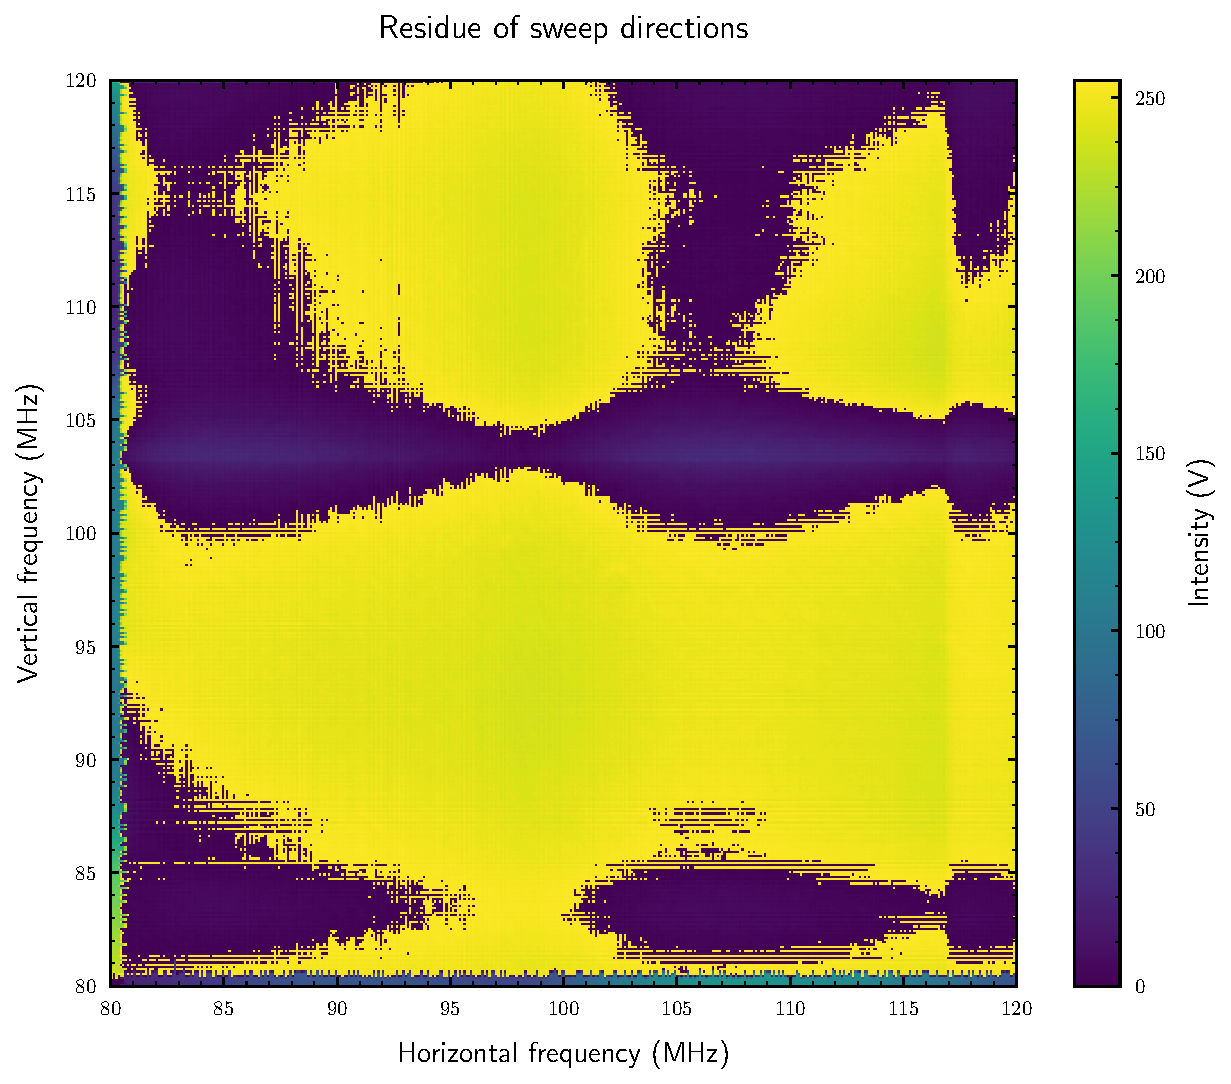
\includegraphics[width=.7\textwidth]{\figuredir{intensity/distribution/paired-frequency-residue.pdf}}
  \captionsetup{width=.9\textwidth}
  \caption{Absolute difference between the 2D intensity distribution
  performed with the digital ramp configured set to different axes.}
  \label{fig:intensity_distribution_frequency_residue}
\end{figure}

As the differences in \Cref{fig:intensity_distribution_frequency} are of only
subtile nature we additionally reveal the absolute difference between both
maps in \Cref{fig:intensity_distribution_frequency_residue}. We observe
nearly a binary map of dark purple and yellow area whereas the dark area can
be intepreted as small and the yellow area as large difference. The binary
nature of the absolute difference reminds us at the fixed offset we observed
between the amplifiers whereas the areas with small difference occur when the
crystal is saturated. However we must admit that this suggestions needs
further evidence.

\subsubsection{Constant sampled frequencies}

In \cref{subsec:signal_synthesizer_amplitude_frequency_response} we found
that the \gls{dds} show a slightly different amplitude frequency response
in the case of frequencies being controlled by the digital ramp. It remains
open if this is also true for the amplifier and in fact even more prominent.

\begin{figure}[ht]
  \centering
  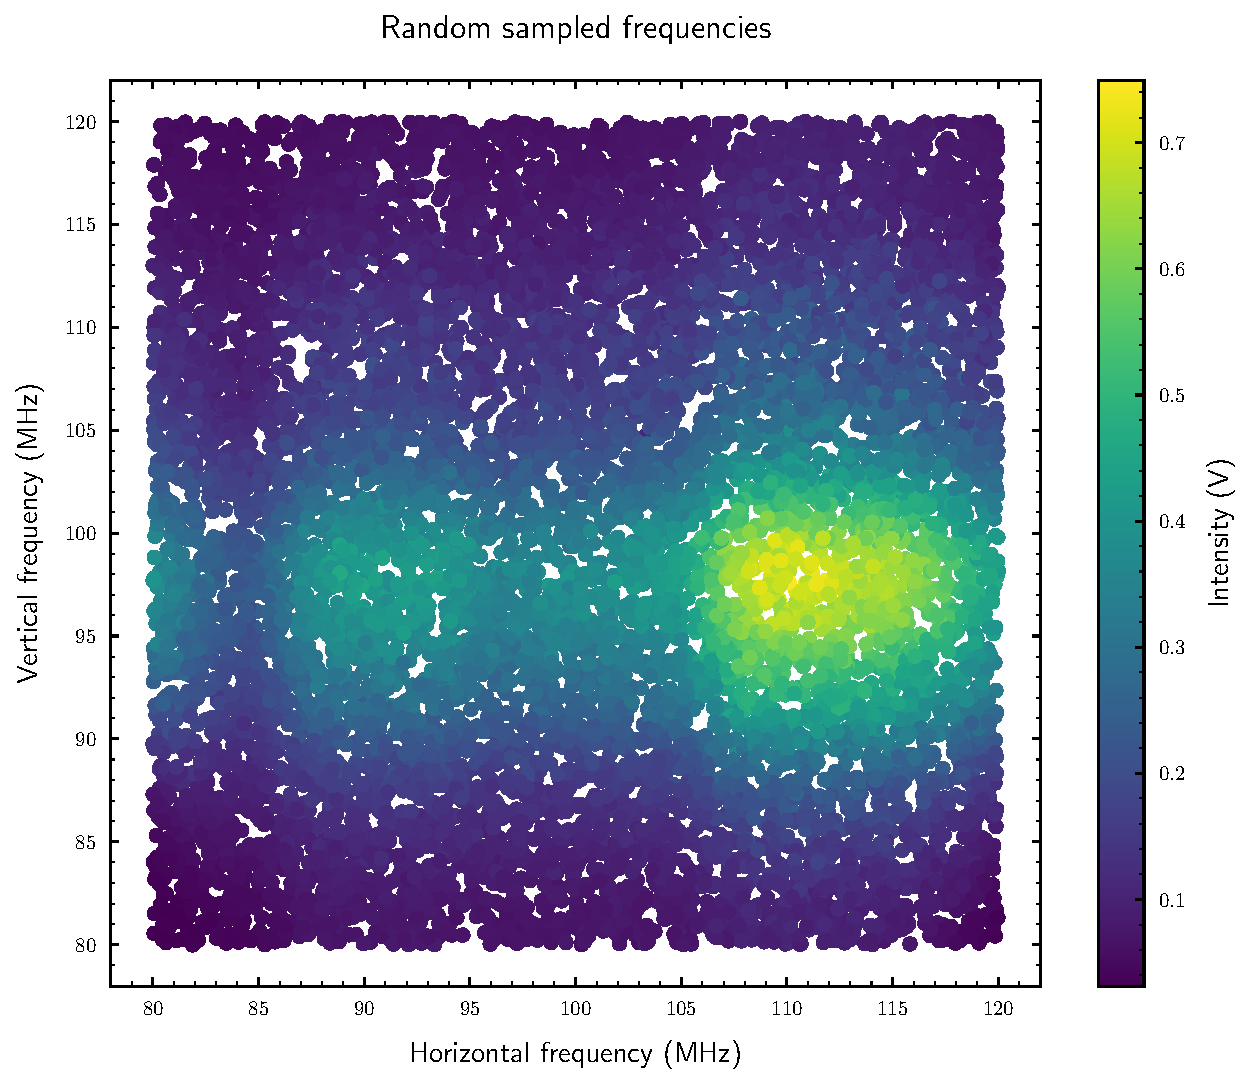
\includegraphics[width=.7\textwidth]{\figuredir{intensity/distribution/sample-frequency.pdf}}
  \captionsetup{width=.9\textwidth}
  \caption{Intensity measured as voltage at the photodiode in dependence of
    the horizontal and vertical applied frequency signal to the \gls{aod}.
    Frequency pairs are sampled over a uniform distribution and then passed
  as constant output frequency paramter to the \gls{dds}.}
  \label{fig:intensity_distribution_frequency_sampled}
\end{figure}

To partly answer this question we sampled random frequency pairs over a
two dimensional uniform distribution and passed them as constant frequency
parameter to the respective \gls{dds}. The yielded intensity distribution
is visualized in \Cref{fig:intensity_distribution_frequency_sampled}. We note
that in comparison to \Cref{fig:intensity_distribution_frequency} the
intensity differences are more concentrated around the vertical axis. This
suggests that there are electronic effects in play during fast sweeps that
do affect the intensity transmission.

\subsubsection{Different radio frequency signal source}

The previous finding suggest that the intensity transmission of the \gls{aod}
is mainly caused by unideal characteristics of the electronic equipment.
Regardless it is still unclear whether the \gls{dds} or the power amplifier
should be held responsible for messing up our signal.

For the following measurement we replaced the vertical \gls{dds} source with
a high-quality signal generator and configured a frequency sweep. We presume
the high-quality signal generator to supply a constant output power level.

\begin{figure}[ht]
  \centering
  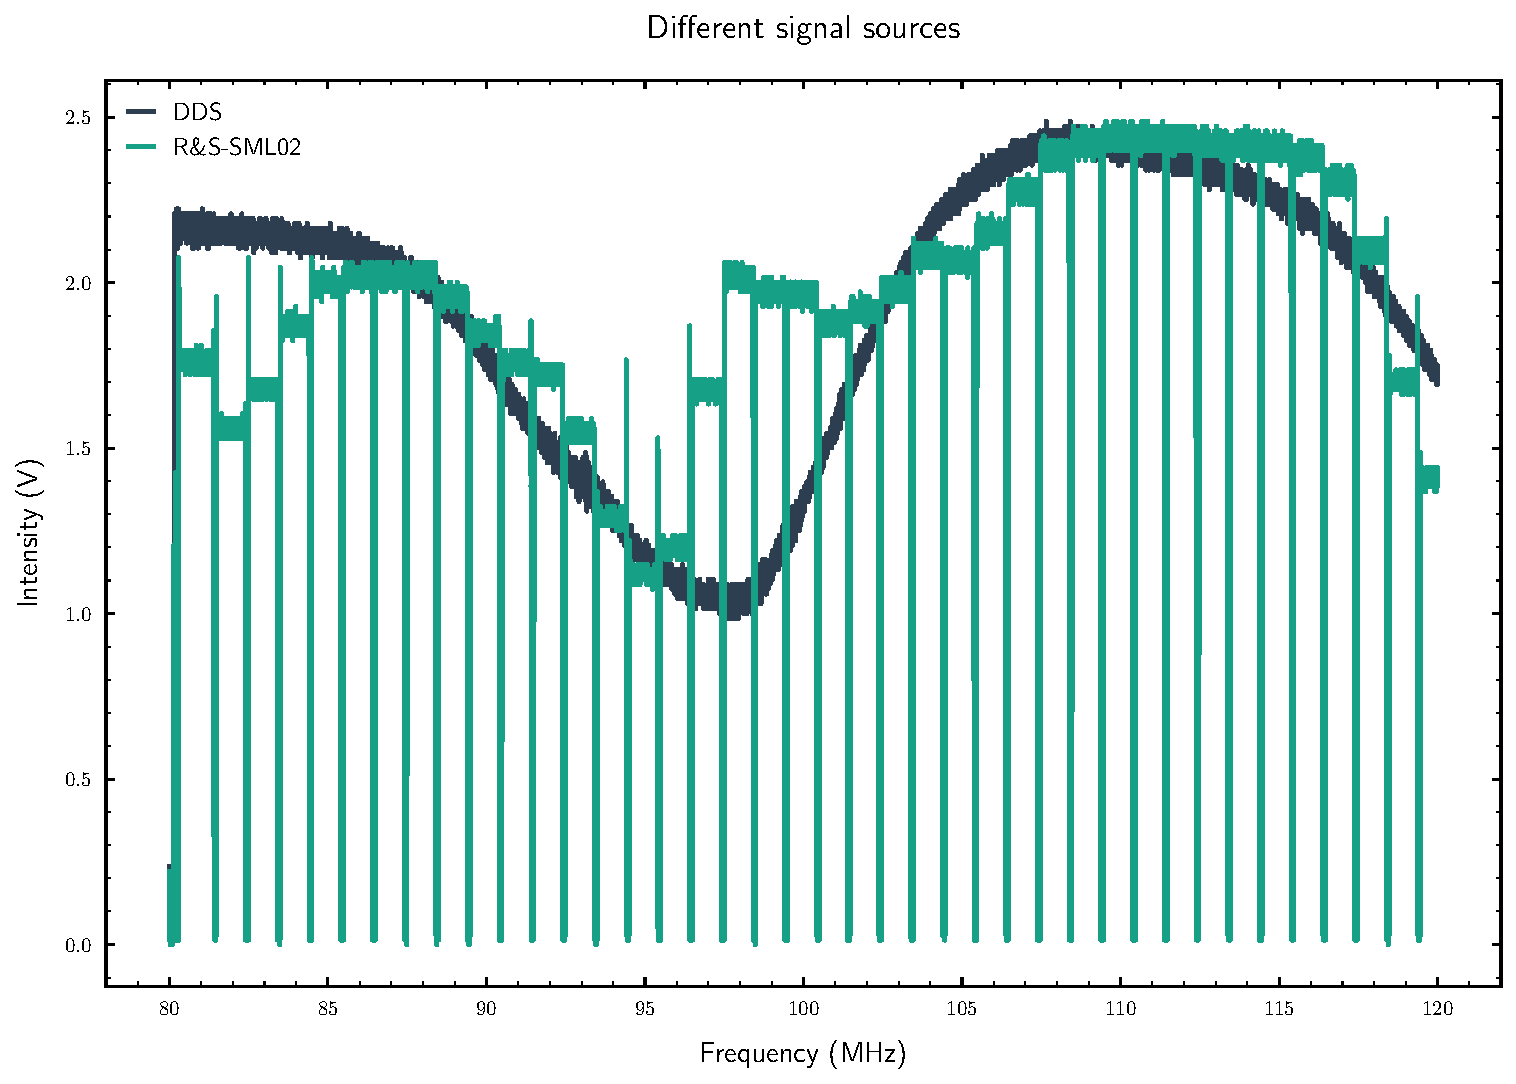
\includegraphics[width=.9\textwidth]{\figuredir{intensity/distribution/signal-sources.pdf}}
  \captionsetup{width=.9\textwidth}
  \caption{Intensity measured as voltage at the photodiode with one \gls{aod}
    at constant center frequency supplied by a \gls{dds} and the other
    \gls{aod} performing a linear frequency sweep with the \gls{dds} and a
  high-quality signal generator.}
  \label{fig:intensity_distribution_signal_sources}
\end{figure}

\Cref{fig:intensity_distribution_signal_sources} discloses the intensity
measured as voltage at the photodiode when the frequency sweep is performed
by two different signal sources and the other \gls{aod} is held at constant
center frequency. We observe that even though the signal generator has a much
more coarse frequency resolution it shares the global characteristics of
the more dense trace from the \gls{dds}. This confirms that the amplifier
seems to be the dominant contributor to the intensity transmission during
frequency sweeps.

\subsubsection{Summary}

In this chapter we found out that the \gls{rf} signal is of major importance
to the observed intensity transmission. In particular the power amplifier
possess a strong frequency power response. The acousto-optics itself seem to
be saturated at some power level. Transmission also seems to differ depending
on the method used to sweep frequencies. All in all there are to many factors
at play to describe with a simple analytical model and we will further try to
not expect much regularities for the optimization procedure in the next
chapter.

\section{Intensity optimization}

The previous two chapters addressed the characteristics of the \gls{rf}
signal and the intensity transmission of the \gls{aod}. Therewith the
groundwork has been set out to finally approach the mission of minimizing the
intensity variance to obtain a homogenous optical potential.

But how do we minimize the intensity variance? The \gls{dds} permit to read
$N=1024$ amplitude values from memory. The optimization problem therefore is to
minimize the variance of the intensity distribution $I(A)$ subject to an
amplitude vector $A\in[0,1]^N$. The conclusions drawn from the intensity
measurements suggest that we have to expect non-linear, irregular behaviour
in $I(A)$. and indeed first attempts to model $I(A)$ through polynomial fits,
multilayer perceptron networks and least-squared minimizations have failed.

During these optimization procedures we observed that changing an amplitude
value $A_i\in A$ does affect the intensity voltage at subsequent
$A_{i+1},\dots,A_N$. Fortunately we found that by respecting the amplitude
order with respect to increasing frequency during optimization we where able
to bypass these effects. Further we created amplitude segments
$\left(A_j,\dots,A_{j+m}\right)$ consisting of $m$ ordered amplitude values
to reduce the optimization time. Optimization then was performed through
random search which was proven to yield better results as grid search
\cite{Bergstra2012}.

\subsubsection{Overview}

First of we want to provide an overview of the final optimization results
obtained at different hyperparameters for the random search. The
hyperparameter include the number of amplitude segments $N/m$ and the target
intensity.

\begin{figure}[ht]
  \centering
  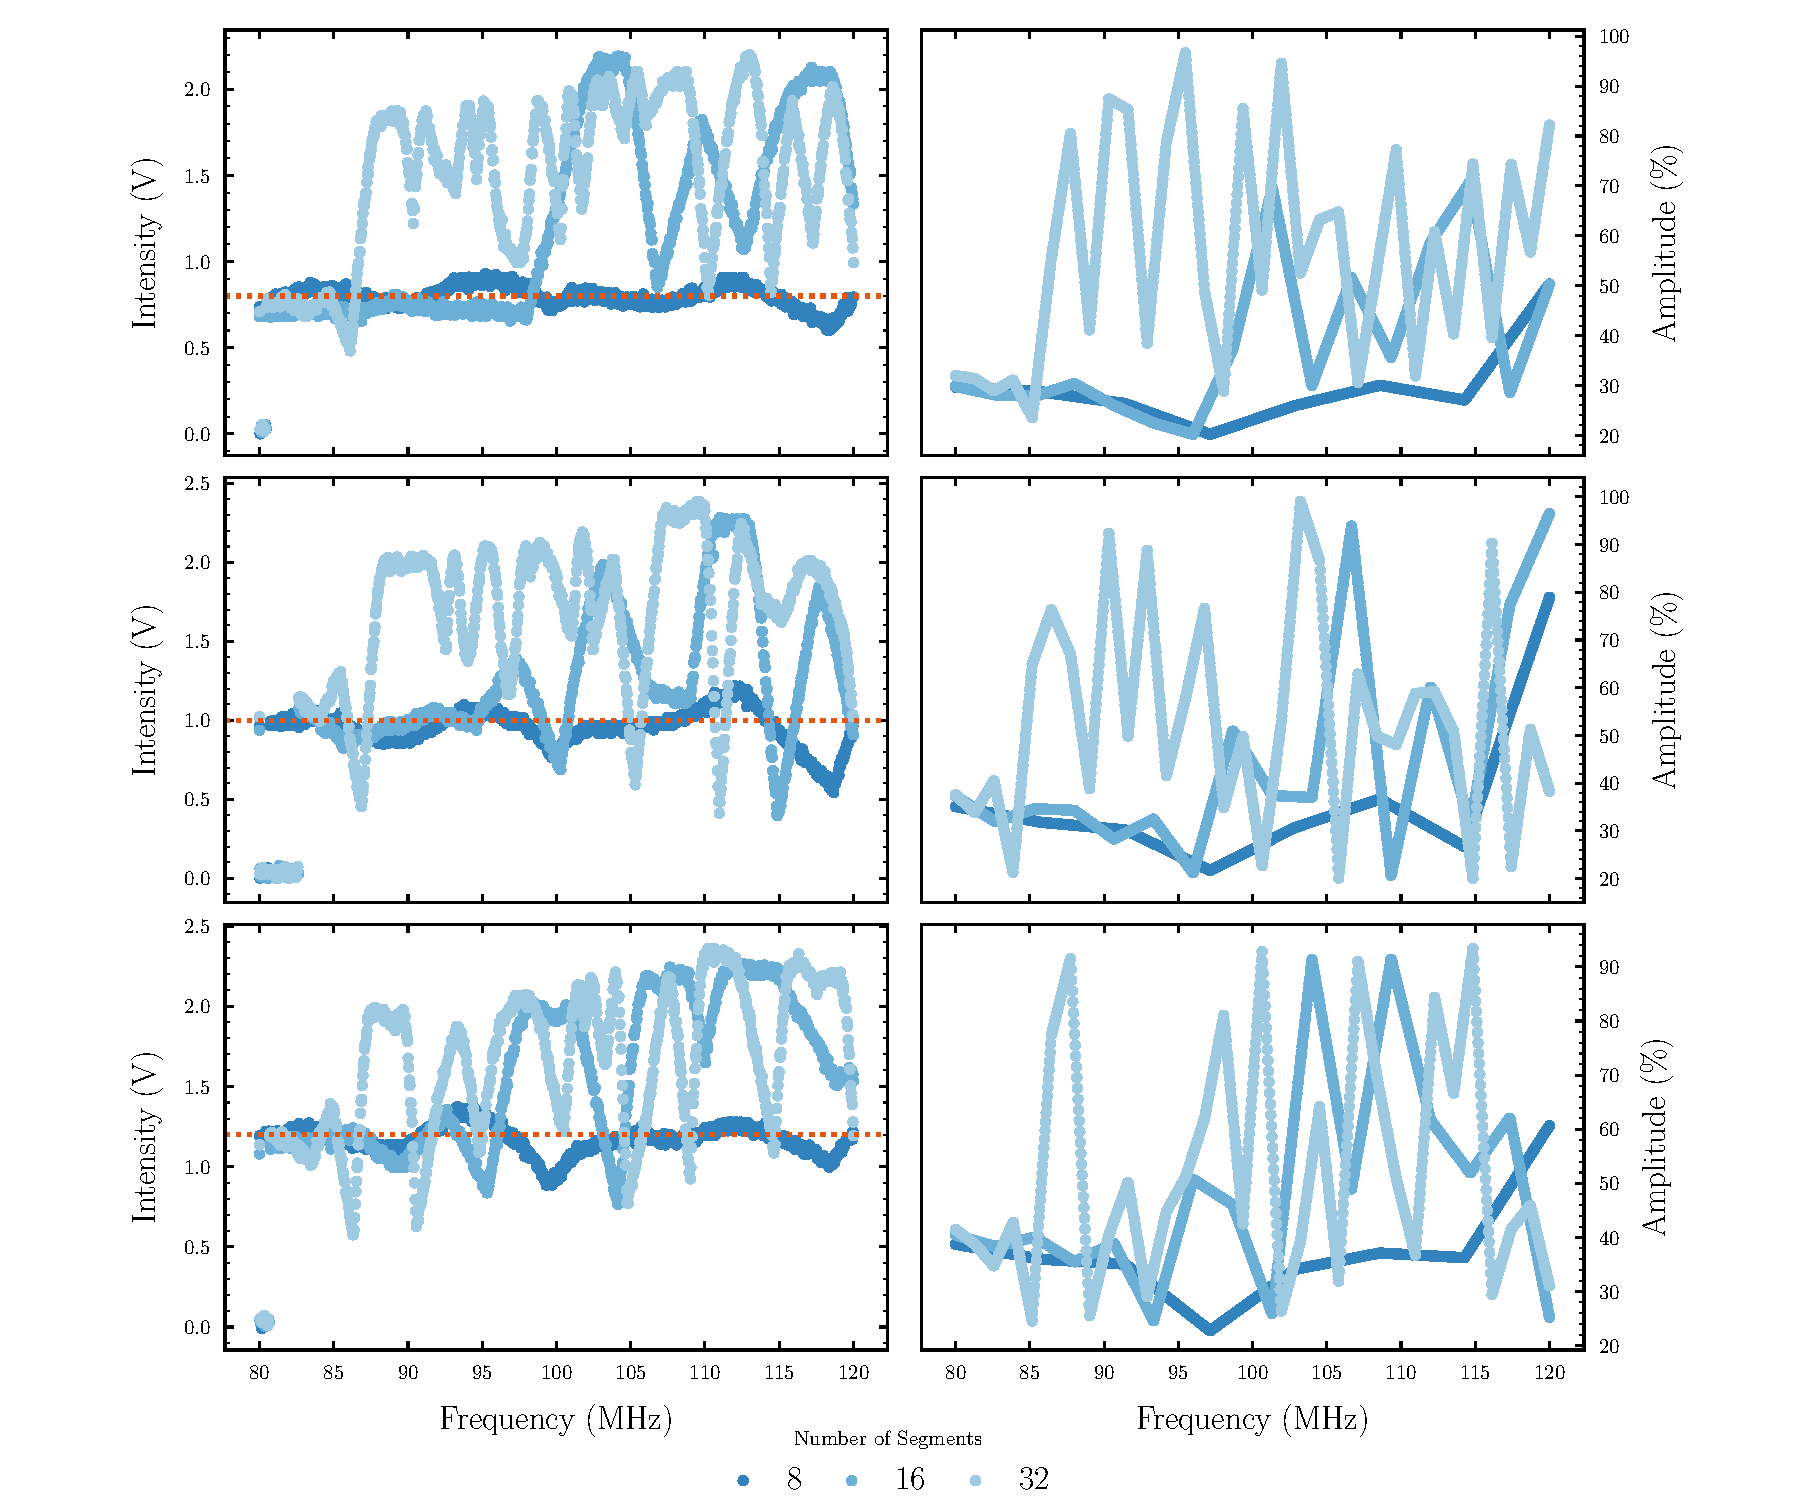
\includegraphics[width=\textwidth]{\figuredir{intensity/optimization/overview.pdf}}
  \captionsetup{width=.8\textwidth}
  \caption{Minimized intensity variance for different target intensities
  and number of amplitude segments. We note heavy oscillations for
  amplitude segments greater than eight.}
  \label{fig:intensity_optimization_overview}
\end{figure}

In \Cref{fig:intensity_optimization_overview} we are presented the final
optimization results for target intensities of \SI{800}{\milli\volt},
\SI{1000}{\milli\volt} and \SI{1200}{\milli\volt} and amplitude segments
$8,16,32$. We observe heavy oscillations for amplitude segments greater than
eight. The optimization results using 16 amplitude segments performs better
than the run with 32 amplitude segments.

We assume that inductive effects occur when choosing more amplitude segments
that consolidate a non-linear intensity response. For the sake of simplicity
we will first limit us to the case of eight amplitude segments.

\begin{figure}[ht]
  \centering
  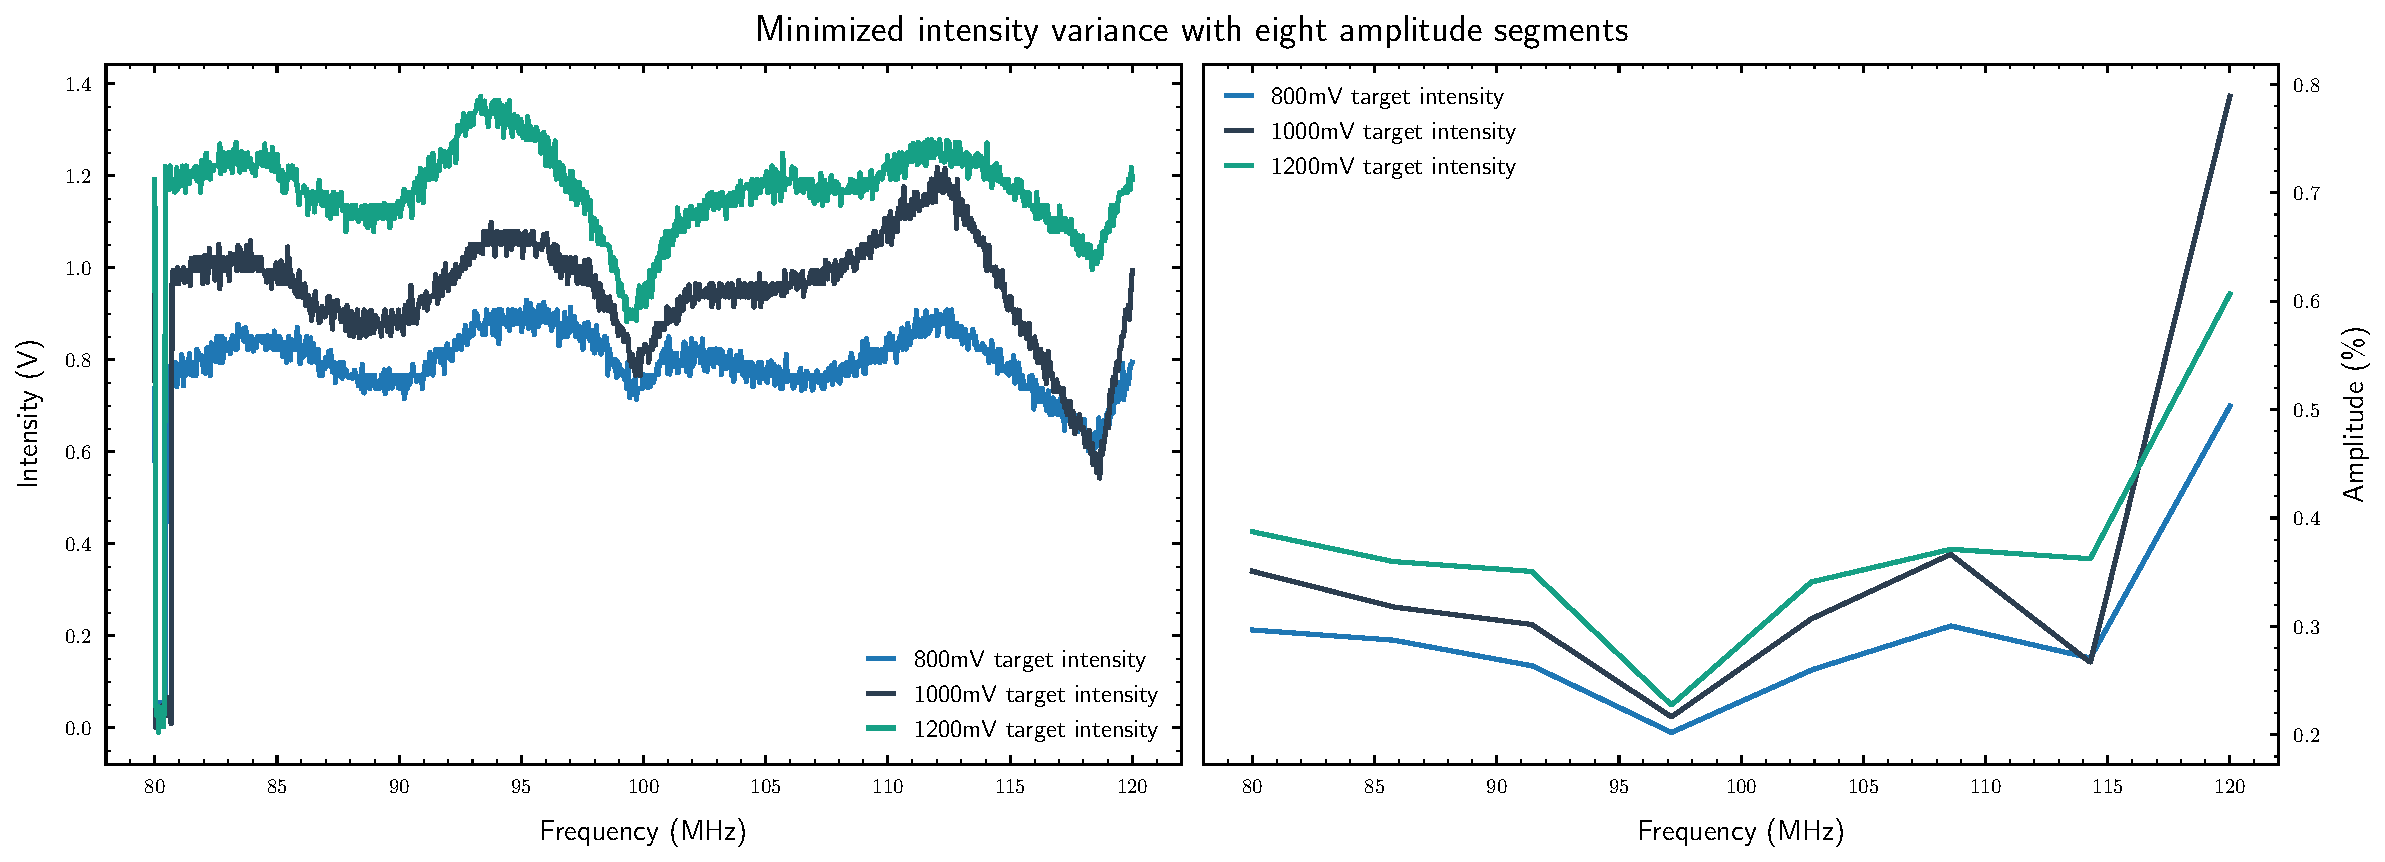
\includegraphics[width=\textwidth]{\figuredir{intensity/optimization/intensity-amplitude.pdf}}
  \captionsetup{width=.8\textwidth}
  \caption{Final result of the intensity variance minimization and the
  corresponding amplitude segment values obtained through random search with
  eight independent amplitude segments.}
  \label{fig:intensity_optimization_intensity_amplitude}
\end{figure}

In \Cref{fig:intensity_optimization_intensity_amplitude} we have a closer
view on the first column of \Cref{fig:intensity_optimization_overview}. We
can notice similar characteristics observed in the \gls{rf} signal. In
particular the more power drop near the center frequency is present and the
linear power fall off with the frequency in the second half of the frequency
sweep.

\subsubsection{Process}

We now want to elaborate on the optimization process. We limit ourselves to
the optimization process with eight amplitude segments as it was the most
successful one and can be covered completly with eight plots.

\begin{figure}[ht]
  \centering
  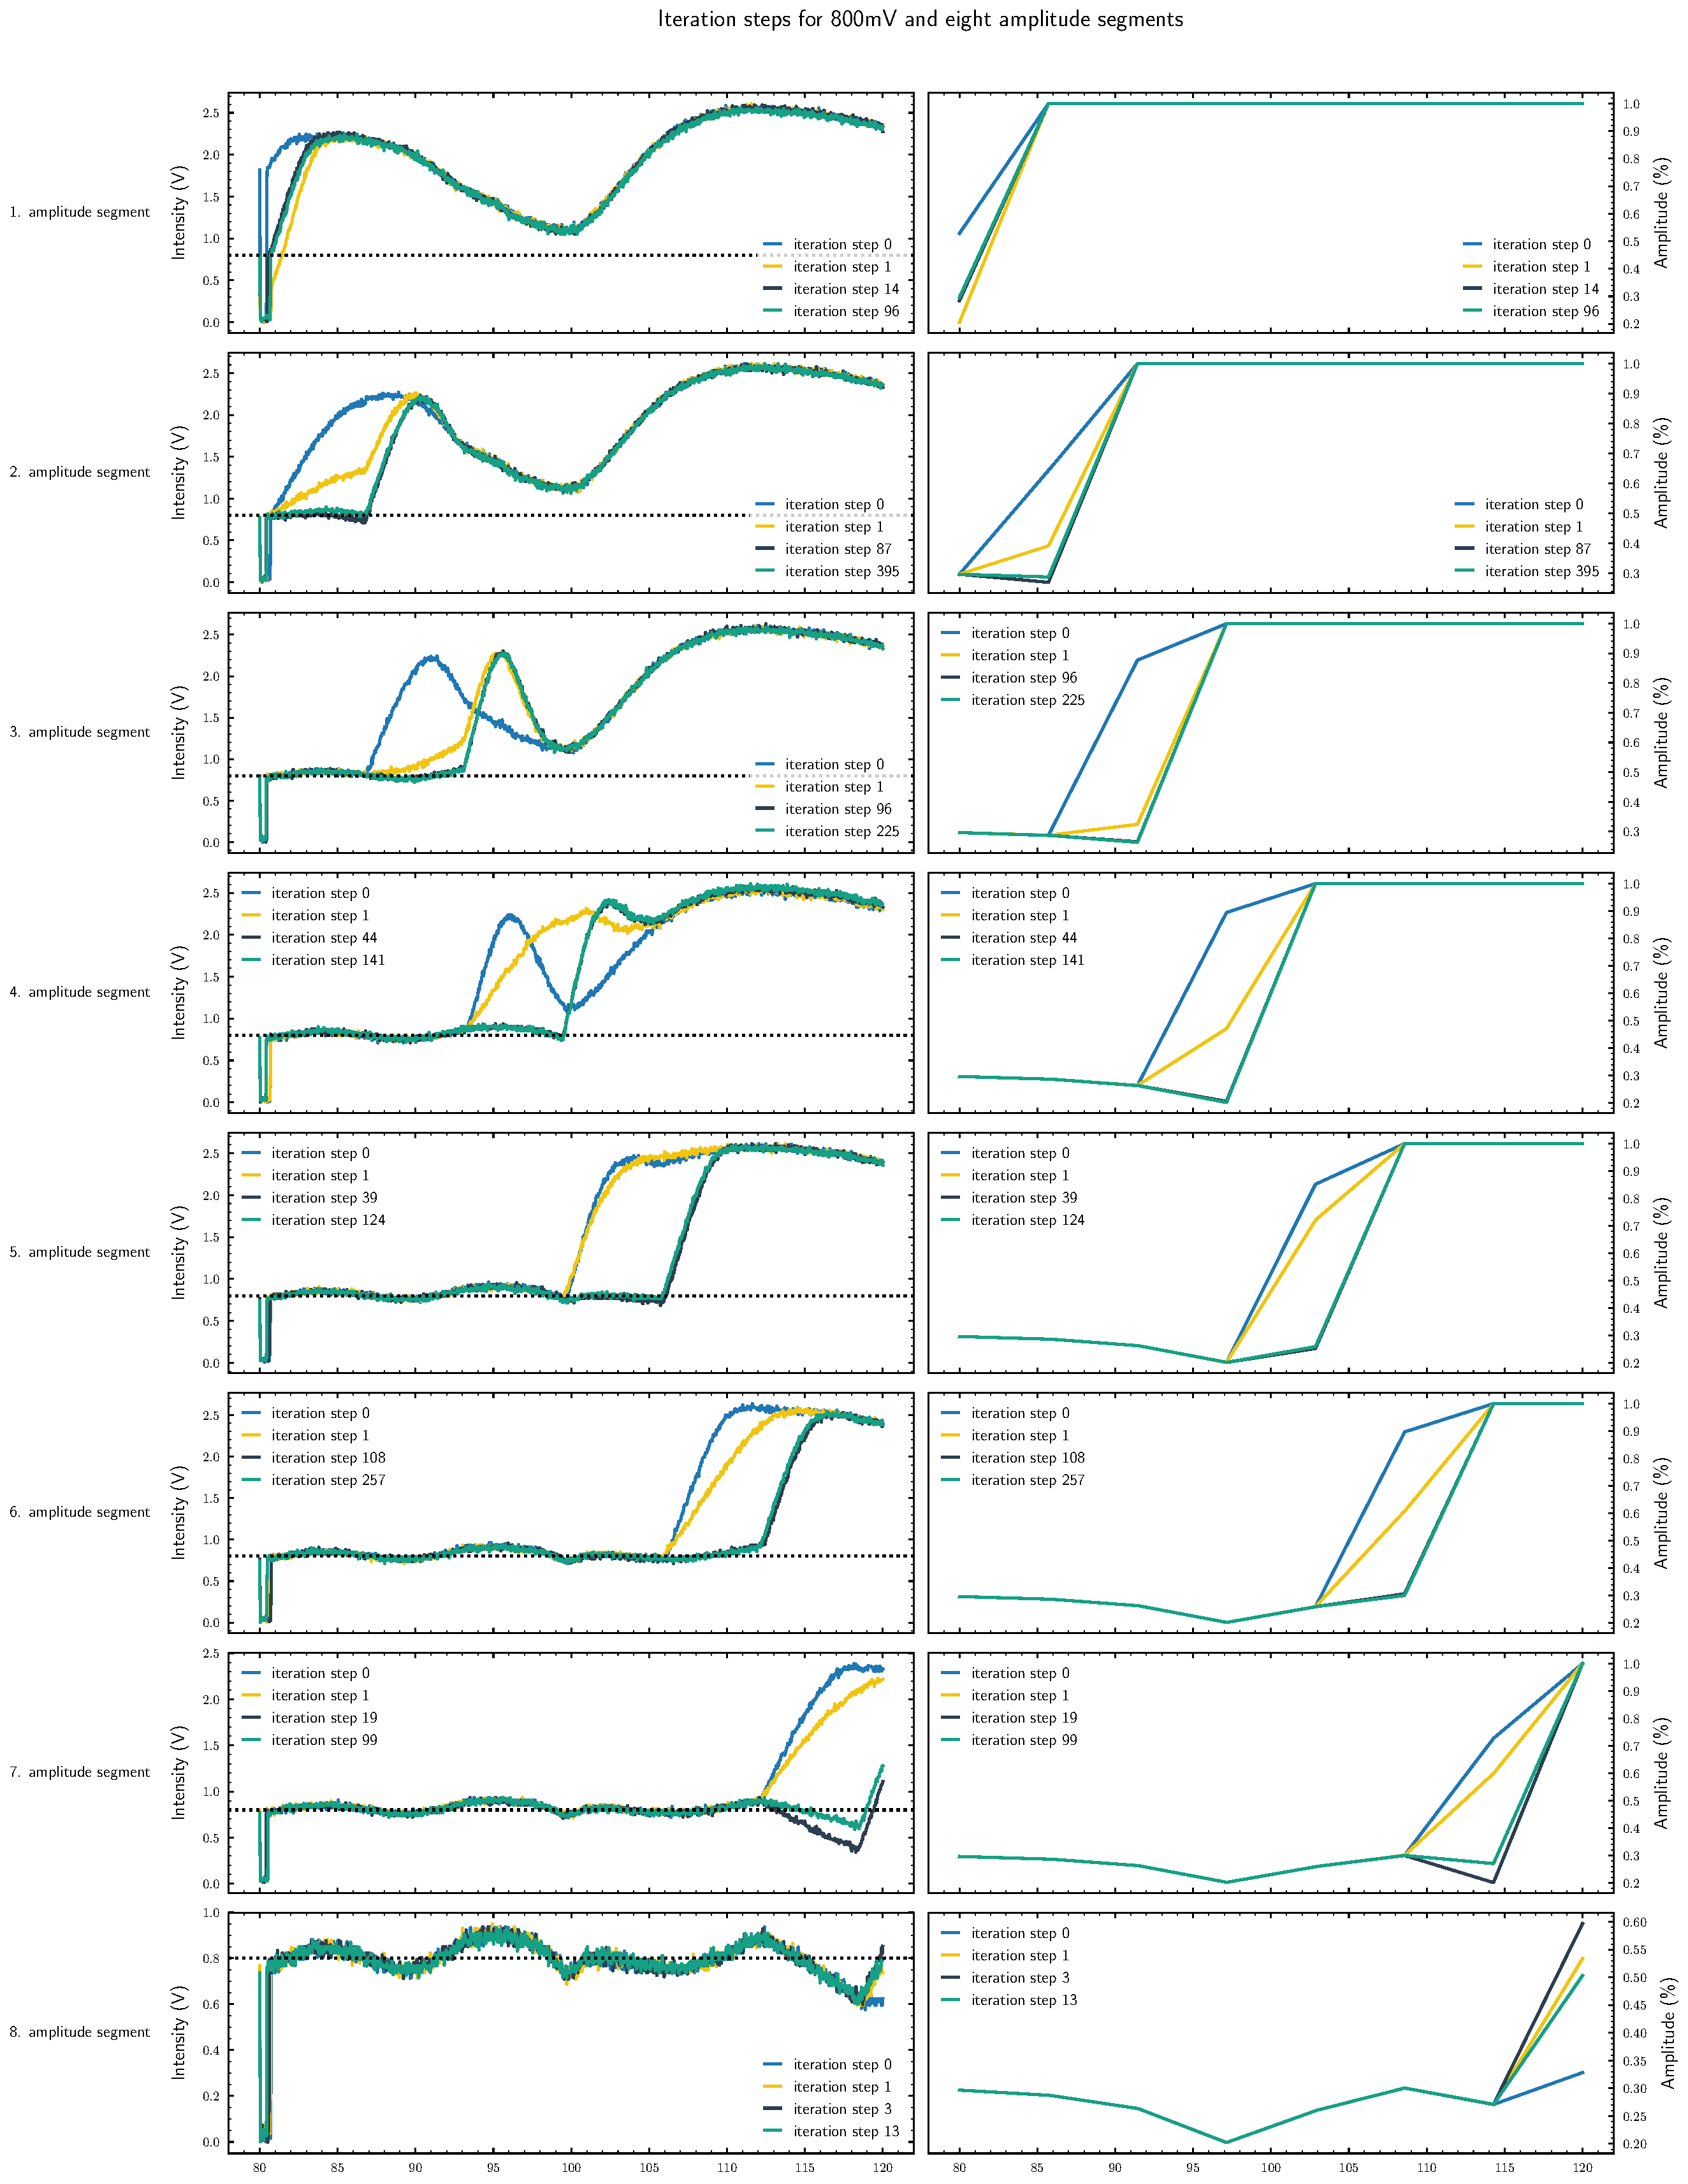
\includegraphics[width=\textwidth]{\figuredir{intensity/optimization/process.pdf}}
  \captionsetup{width=.8\textwidth}
  \caption{Intensity and amplitude at different stages of the optimization
  process. In each column a different amplitude segment is optimized.
  The different traces in each plot mark the respective iteration.}
  \label{fig:intensity_optimization_process}
\end{figure}

In \Cref{fig:intensity_optimization_process} we see the intensity and
amplitude at different optimization stages. At each stage one amplitude
segment is sampled from a uniform distribution over $[.2, .8]$. The intensity
segment associated with this amplitude segment is then used to calculate
the \gls{mse} and compare it to the previous best \gls{mse}. If the new
\gls{mse} is less than the previous best \gls{mse} the previous best \gls{mse}
is updated and the amplitude segment value is saved. This procedure is
repeated 500 times. Every time a new best value was found we saved the
data. For the diagrams we choose the four most separated iteration steps to
visualize the process of the optimization.

If we take a look at the succeeding segment from the currently optimized
amplitude segment we observe that these differ for different amplitude
values and henceforth confirms that amplitude values are not independent but
affect subsequent segments.

\subsubsection{Failure}

With the optimization showing reasonable convergence for eight amplitude
segments we would expect it to improve if we choose a more amplitude segments,
yet we observed heavy oscillations. In this section we want to check the
optimization process in the case of 32 amplitude segments to investigate in
possible origins of the optimization failure.

\begin{figure}[ht]
  \centering
  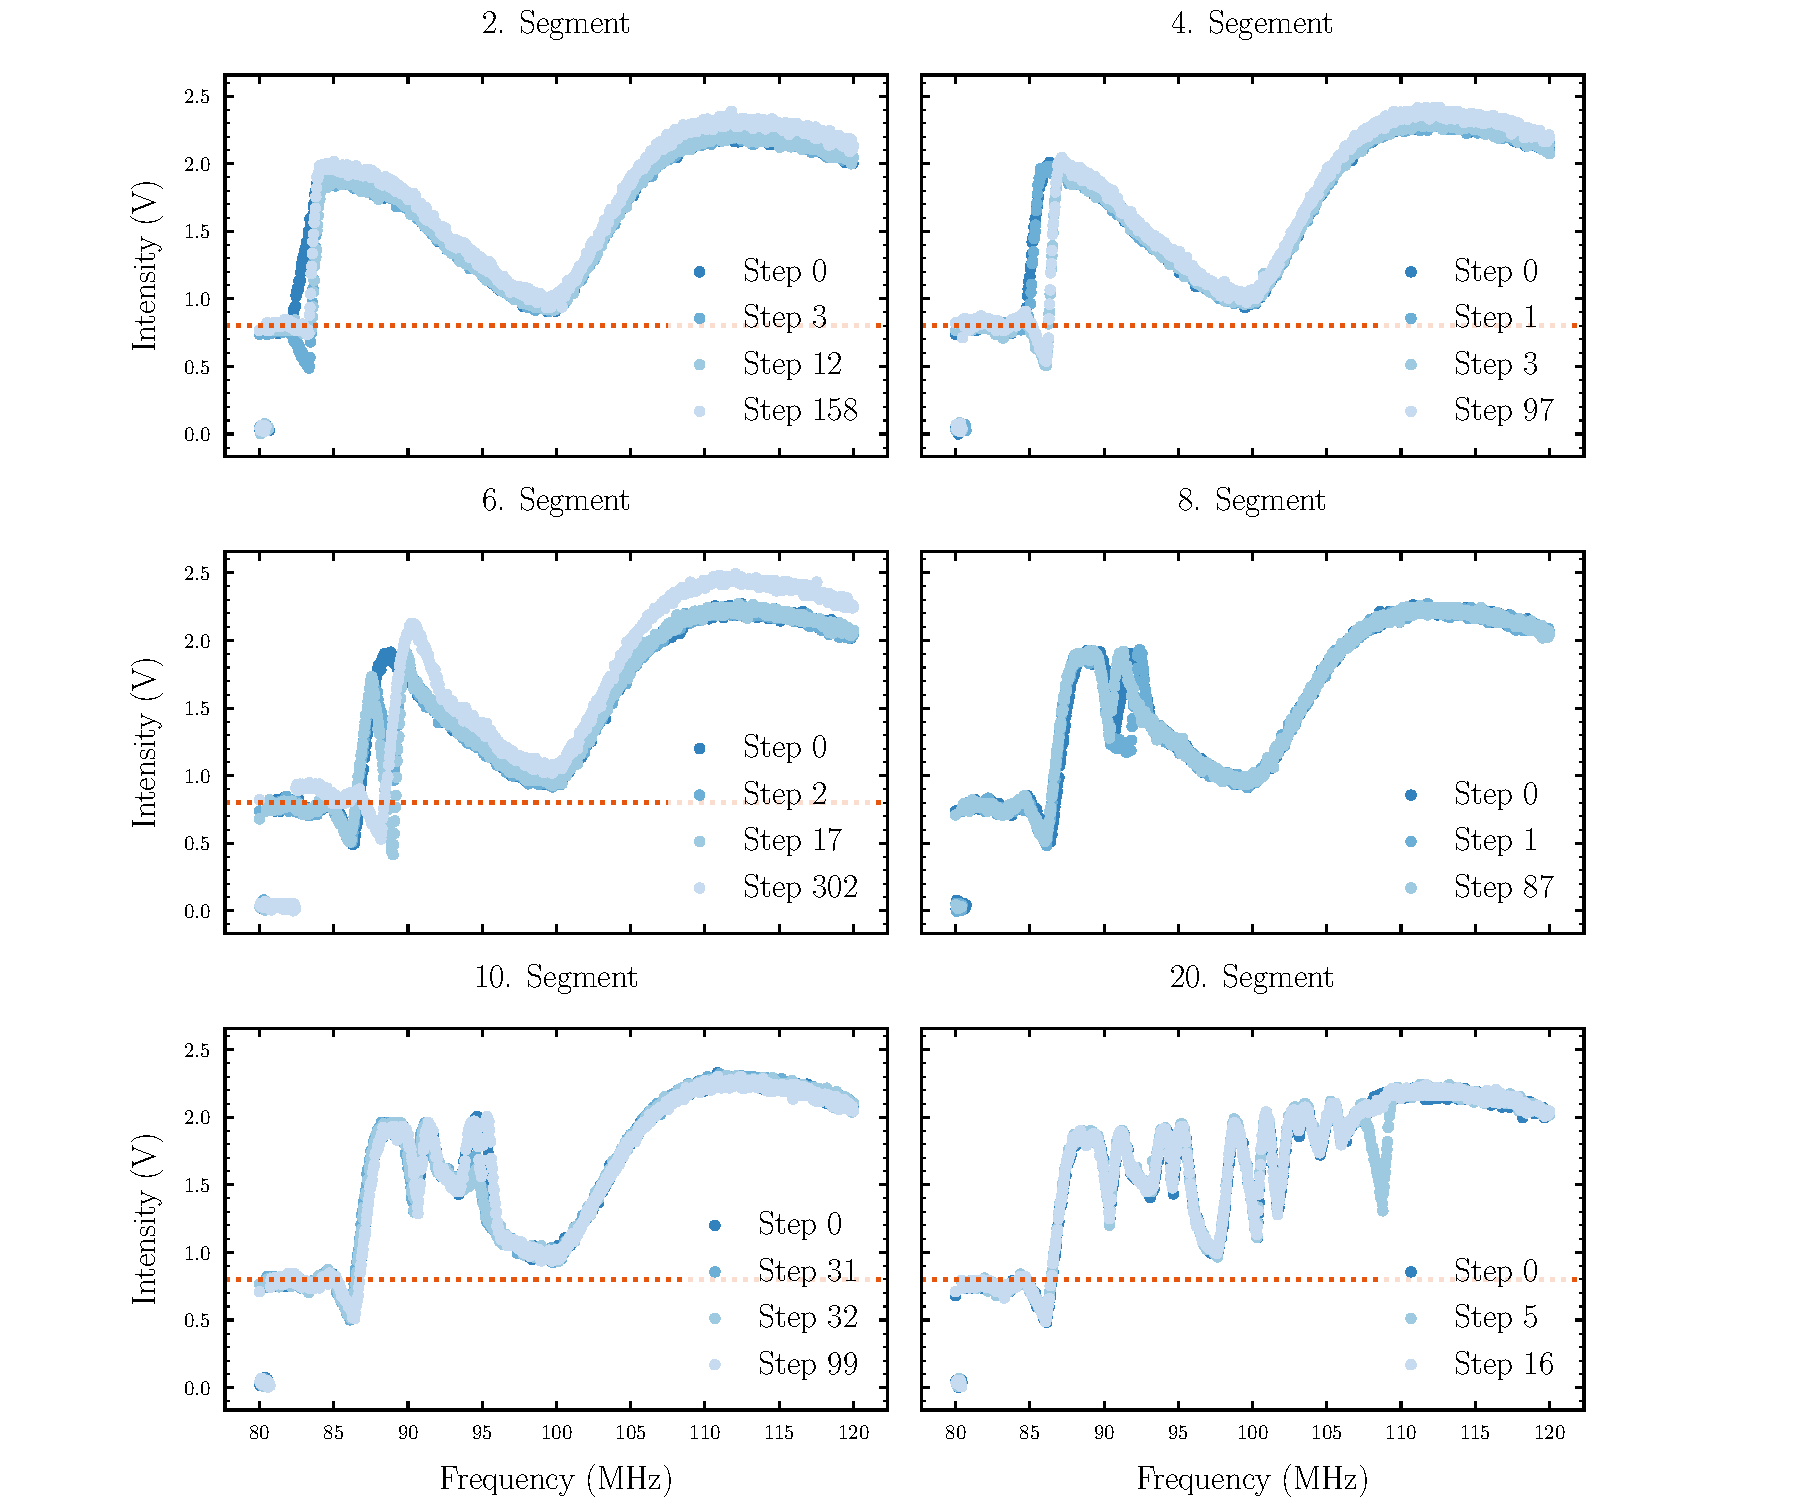
\includegraphics[width=\textwidth]{\figuredir{intensity/optimization/failure.pdf}}
  \captionsetup{width=.8\textwidth}
  \caption{Optimization progress for the 2.,4.,6.,8.,10. and 20. amplitude
  segment of the failed optimization run with 32 amplitude segments. We can
  see that with increasing amplitude segments the non-linear response
  following the optimized amplitude segment increases.}
  \label{fig:intensity_optimization_failure}
\end{figure}

In \Cref{fig:intensity_optimization_failure} we can see the optimization
progress for selected amplitude segments of the optimization run with 32
segments. We observe that with the non-linear response following the actual
optimized amplitude segment increases more and more.

\subsubsection{Summary}

Our attemps to minimize the intensity variance where of mixed success. One
the one hand side we were able to minimize the intensity deviation down
to \SI{100}{\milli\volt} on the other hand we were not able to train any
model on the intensity response that would allow fast optimization or even
predicition of the expected intensity response given an amplitude
configuration.

However we also found out that irregularities arise with increase in the
number of amplitude segments. We suspect that fast changes of the output
amplitude draws power that may non deterministicyl affect the next clock
cycle inside the \gls{dds}. Given that the one dimensional optimizations
already required multiple hours to run and the non-linear response between
amplitude segments we do not believe that it is not in the capabilites of the
\gls{dds} to compensate for the two dimensional intensity distribution
measured in the previous chapter.
